\chapter{Results\label{ch:results}}

After applying the preselection, event classification, and mass windows, signal efficiency
and event yields are examined. This is detailed in Section~\ref{sec:yields}. Then, signal yield
in data is evaluated through the calculation of the confidence level (CL)
for exclusion or for discovery of double Higgs production is evaluated from a simultaneous fit
to the $\Mgg$, $\Mggjjk$, or $\Mgg \times \Mjj$ specta for the low-mass resonant, high-mass resonant,
or nonresonant searches, respectively.
To compute the upper limits on the production cross section, the modified frequentist approach
$\text{CL}_s$ is used with an asymptotic approximation, taking thee profile likelihood as a test
statistic~\cite{CLS1,CLS2}. This calculation is discussed in Sections~\ref{sec:resresults} for the
resonant search and in Section~\ref{sec:nonresresults} for the SM nonresonant search.

\section{Signal Efficiencies and Yields\label{sec:yields}}

The signal effiency as a function of $m_X$ for the resonant search is summarized in
Figure~\ref{fig:eff_res}. The signal efficiency increases from 260 GeV to 900 GeV
from better photon and jet reconstruction efficiencies. The signal efficiency
peaks at and drops after 900 GeV due to the merging of the two jets from the decay $\Hbb$ into
a single jet. For future consideration in extending the search above 1.1 TeV,
through jet substructure techniques would be necessary to resolve the jet merging~\cite{Ellis:2009su}.
Both categories contribute approximately equally to the overall efficiency.

\begin{figure}[ht]
 \begin{center}
    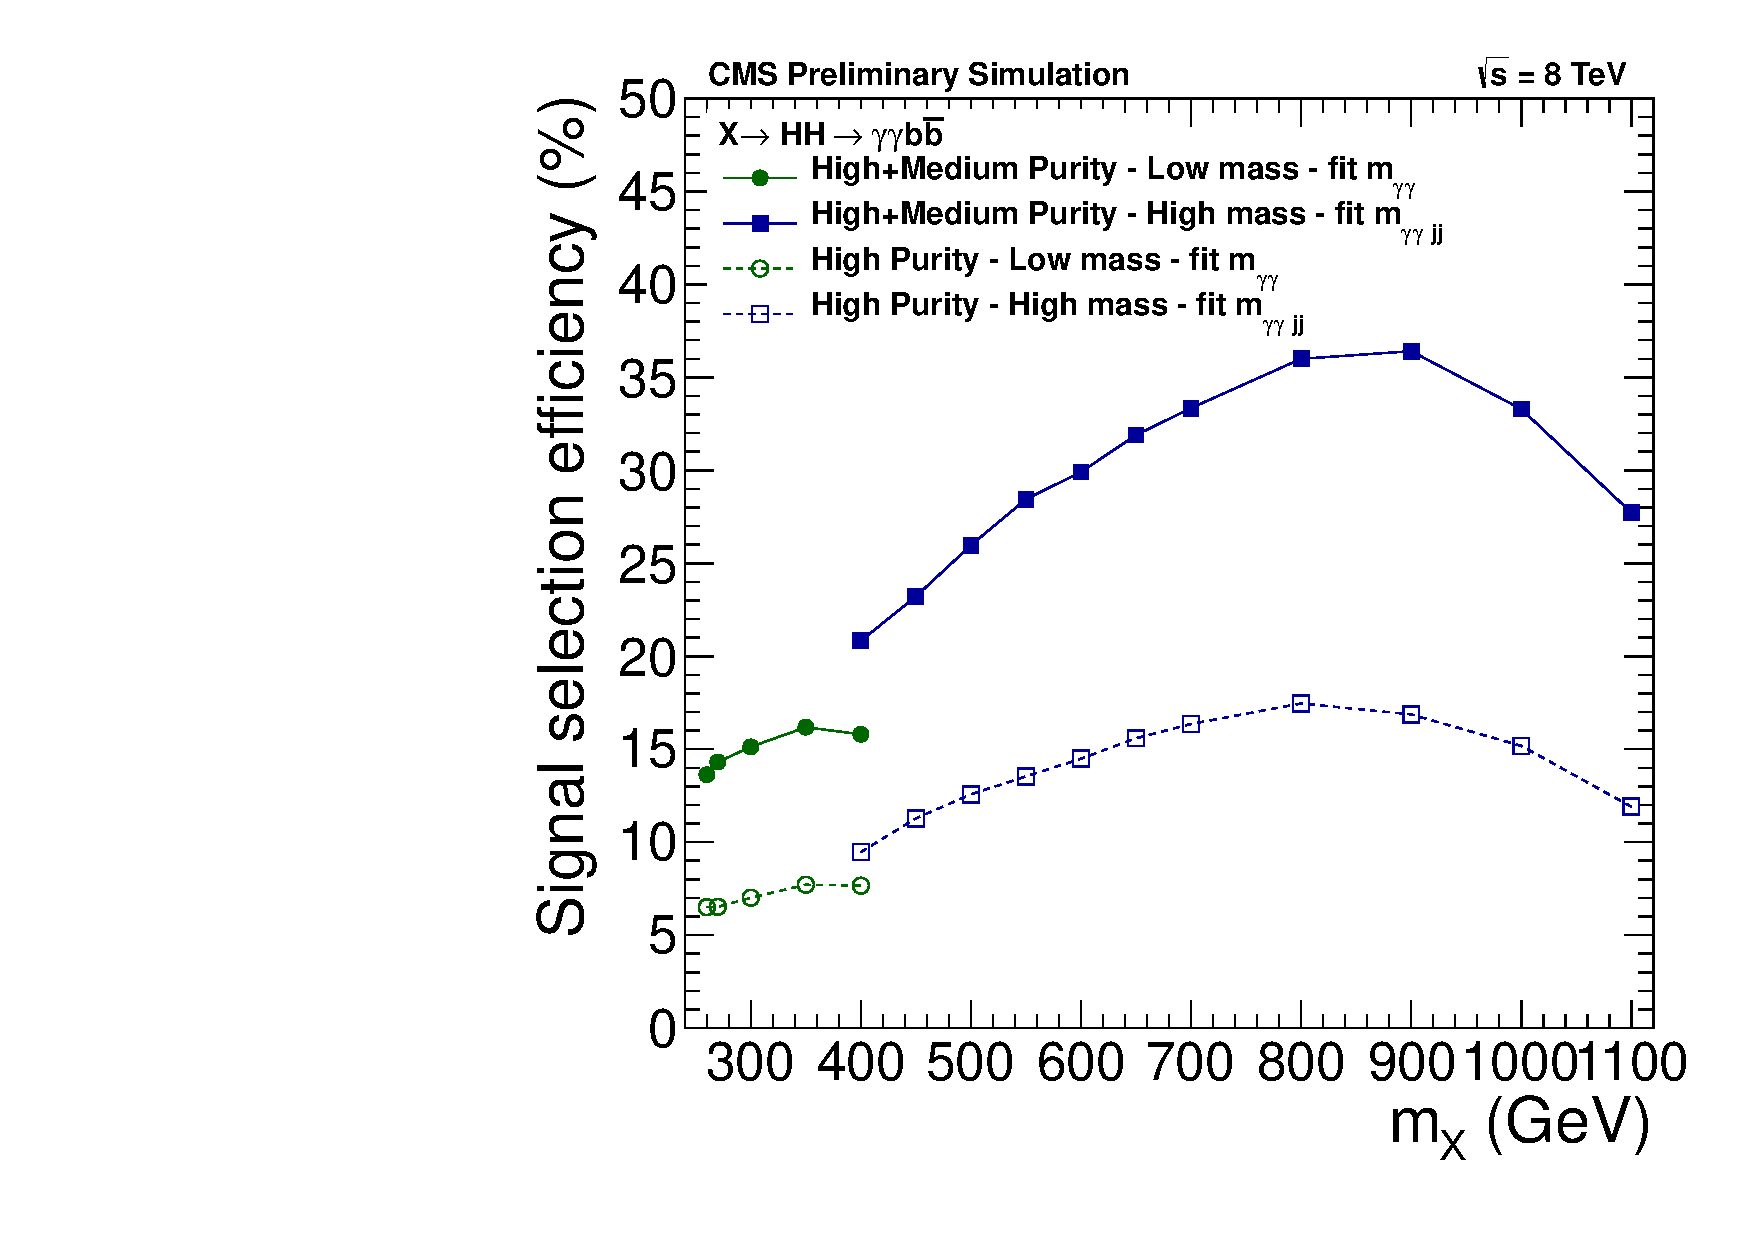
\includegraphics[width=0.70\textwidth]{figures/results/eff_all.pdf}
      \end{center}
\caption{Signal efficiency for the resonant search for final selection.}
\label{fig:eff_res}
\end{figure}

The yields for the low-mass resonant search at $m_X = 300$~GeV are summarized in
Table~\ref{table:yield_lowmass_res}. Note that there is a normalization disagreement in the
$\gamma\gamma j$ and $\gamma j$ contributions as the simulation has limitations in modeling
QCD with one or two hard photons. As a result, the backgrounds are not added; the purpose is to
highlight relative contributions. The yields for the high-mass resonant search are summarized in
Table~\ref{table:yield_highmass_res}. For this search, the requirements are independent of
the mass hypothesis, so a several signal hypotheses can be shown together.

\begin{table}[ht]
  \centering
  \renewcommand{\arraystretch}{1.4}
  \caption{Event yields for the low-mass resonant search at 300 GeV. Expectations are given for
the signal, resonant background, and nonresonant background. Counts are given for data. Note that
there is a normalization disagreement coming from the shortcomings of simulating QCD with one
or two hard photons.}
  \begin{tabular}{|c|c|c|}
\hline
Sample & High purity & Medium purity\\
\hline
Radion (300$~$GeV, $\Lambda_R$=1TeV)  & 18.73 & 21.66     \\
\hline
ggF $\Hgg$                &  0.02  &  0.19 \\
VBF $\Hgg$                &  0.00  &  0.04 \\
$WH(\gamma\gamma)$        &  0.00  &  0.05 \\
$ZH(\gamma\gamma)$        &  0.00  &  0.03 \\
$t\bar{t}H(\gamma\gamma)$ &  0.10  &  0.15 \\
\hline
$\gamma\gamma j$                      & 8.9  &  188  \\
$\gamma j$                            & 0.00 &  9.2  \\ 
QCD                                   & 0.00 &  0.00 \\ 
$Z/\gamma^*\rightarrow\ell^+\ell^- + Z(\ell^+\ell^-)\gamma + W(\ell\nu)\gamma\gamma$ & 0.00 &  0.21 \\
$t\bar{t}\gamma\gamma + t\gamma\gamma + t\bar{t}\gamma j$ & 0.44 &  1.2  \\
\hline
Data                                  & 21 & 230 \\
\hline
\end{tabular}

  \label{table:yield_lowmass_res}
\end{table}

\begin{table}[ht]
  \centering
  \renewcommand{\arraystretch}{1.4}
  \caption{Event yields for the high-mass resonant search. Expectations are given for
the signal, resonant background, and nonresonant background. Counts are given for data. Note that
there is a normalization disagreement coming from the shortcomings of simulating QCD with one
or two hard photons.}
  \begin{tabular}{|c|c|c|}
\hline
Sample & High purity & Medium purity\\
\hline
Radion (500$~$GeV, $\Lambda_R$=1TeV)        &  6.08  & 6.47     \\
Radion (700$~$GeV, $\Lambda_R$=1TeV)        &  2.92  & 3.03     \\
Radion (1000$~$GeV, $\Lambda_R$=1TeV)       &  0.94  & 1.12     \\
\hline
ggF $\Hgg$                &  0.07  &  0.6  \\
VBF $\Hgg$                &  0.01  &  0.12 \\
$WH(\gamma\gamma)$        &  0.00  &  0.10 \\
$ZH(\gamma\gamma)$        &  0.03  &  0.07 \\
$t\bar{t}H(\gamma\gamma)$ &  0.24  &  0.50 \\
\hline
$\gamma\gamma j$                      & 3.0  &  70   \\
$\gamma j$                            & 0.00 &  3.0  \\
QCD                                   & 0.00 &  0.00 \\
& 8.9  &  188  \\
& 0.00 &  9.2  \\ 
& 0.00 &  0.00 \\ 
$Z/\gamma^*\rightarrow\ell^+\ell^- + Z(\ell^+\ell^-)\gamma + W(\ell\nu)\gamma\gamma$ & 0.00 &  0.08 \\
$t\bar{t}\gamma\gamma + t\gamma\gamma + t\bar{t}\gamma j$ & 0.15 &  0.55 \\
\hline
Data                                  & 8 & 79 \\
\hline
\end{tabular}

  \label{table:yield_highmass_res}
\end{table}

The yields for the nonresonant search are summarized in Table~\ref{table:yield_nonres}.
The yields are higher in the nonresonant search because the $\Mggjjk$ spectrum is much less
disciminating than in the low-mass resonant search and because the $\Mjj$ is fit rather than
selected.

\begin{table}[ht]
  \centering
  \renewcommand{\arraystretch}{1.4}
  \caption{Event yields for the nonresonant search. Expectations are given for
the SM nonresonant signal, resonant background, and nonresonant background.
Counts are given for data. Note that
there is a normalization disagreement coming from the shortcomings of simulating QCD with one
or two hard photons.}
  \begin{tabular}{|c|c|c|c|c|}
\hline
 & \multicolumn{2}{c|}{High Purity} & \multicolumn{2}{c|}{Medium Purity} \\
Sample & high $\Mggjjk$ & low $\Mggjjk$ & high $\Mggjjk$ & low $\Mggjjk$ \\
\hline
SM nonresonant $HH$ & 2.03 & 0.28 & 1.99 & 0.20\\
%SM: $\kapl = 1$, $\kapt = 1$, $\ctwo = 0$ & 2.03 & 0.28 & 1.99 & 0.20\\
%$\kapl = 20$, $\kapt = 1$, $\ctwo = 0$ & 78.7 & 102 & 86.5 & 96.5\\
%$\kapl = 1$, $\kapt = 1$, $\ctwo = -2$  & 103 & 16.2 & 101 & 16.5\\
%lam=1  yt=1 c2=0  xsec = 9.96
%lam=20 yt=1 c2=0  xsec = 1046
%lam=1  yt=1 c2=-2 xsec  = 511
\hline
ggF $\Hgg$                &  0.05 & 0.04 & 0.29 & 0.32\\
VBF $\Hgg$                &  0.01 & 0.01 & 0.05 & 0.05\\
$WH(\gamma\gamma)$        &  0.00 & 0.00 & 0.12 & 0.09\\     
$ZH(\gamma\gamma)$        &  0.04 & 0.02 & 0.07 & 0.05\\
$t\bar{t}H(\gamma\gamma)$ &  0.16 & 0.17 & 0.30 & 0.17\\
$b\bar{b}H(\gamma\gamma)$ &  0.00 & 0.01 & 0.01 & 0.04\\  
\hline
$\gamma\gamma j$     &  13 & 21  & 151 & 268 \\
$\gamma j$           & 0.00& 4.3 & 28  & 53  \\
QCD                  & 0.00& 0.00& 0.00& 0.00\\
$Z/\gamma^*\rightarrow\ell^+\ell^- + Z(\ell^+\ell^-)\gamma + W(\ell\nu)\gamma\gamma$
   & 0.00 & 0.01 & 2.3 & 0.18 \\
$t\bar{t}\gamma\gamma + t\gamma\gamma + t\bar{t}\gamma j$ &  1.3 & 2.2 & 3.3 & 3.4 \\
\hline
Data                                  & 41 & 136 & 37 & 319 \\
\hline
\end{tabular}

  \label{table:yield_nonres}
\end{table}

\section{Resonant Results\label{sec:resresults}}

\subsection{Low-mass Resonant Results}

For the low-mass resonant search, the signal yield is extracted by fitting the $\Mgg$ spectrum.
The signal model is built for each mass hypthesis by fitting the $\Mgg$ peak in the simulation sample
separately for the two categories. The functional form used is the sum of a Crystal Ball and
Gaussian with the means constrained to be the same,
where the former models the core of the distribution and the latter models the
tails. The position of the peak and the spread having no dependence on the resonant mass and the
category. Figure~\ref{fig:sigfit_300} shows an example of the signal fit for a mass hypothesis 300 GeV.

\begin{figure}[ht]
 \begin{center}
   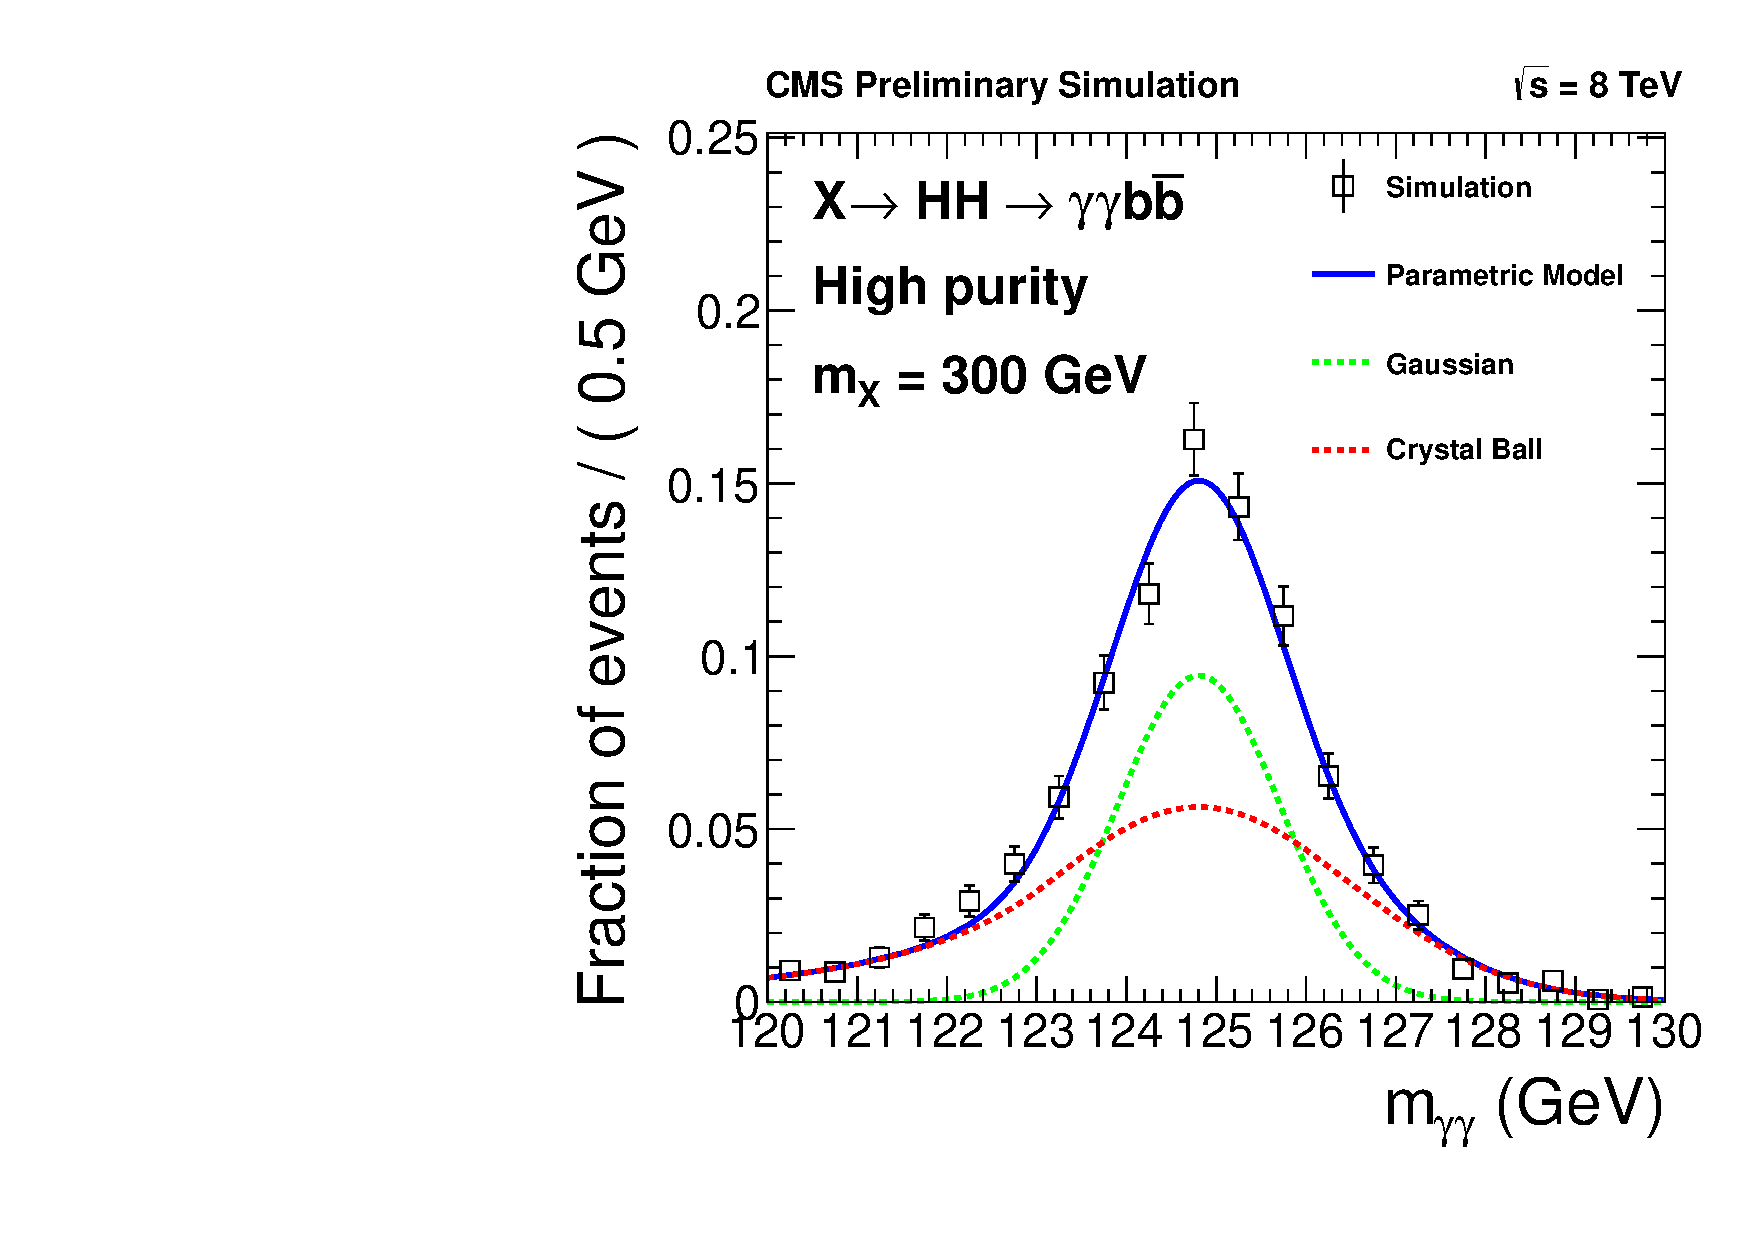
\includegraphics[width=0.70\textwidth]{figures/results/sigmodel_cat0_300.pdf}
   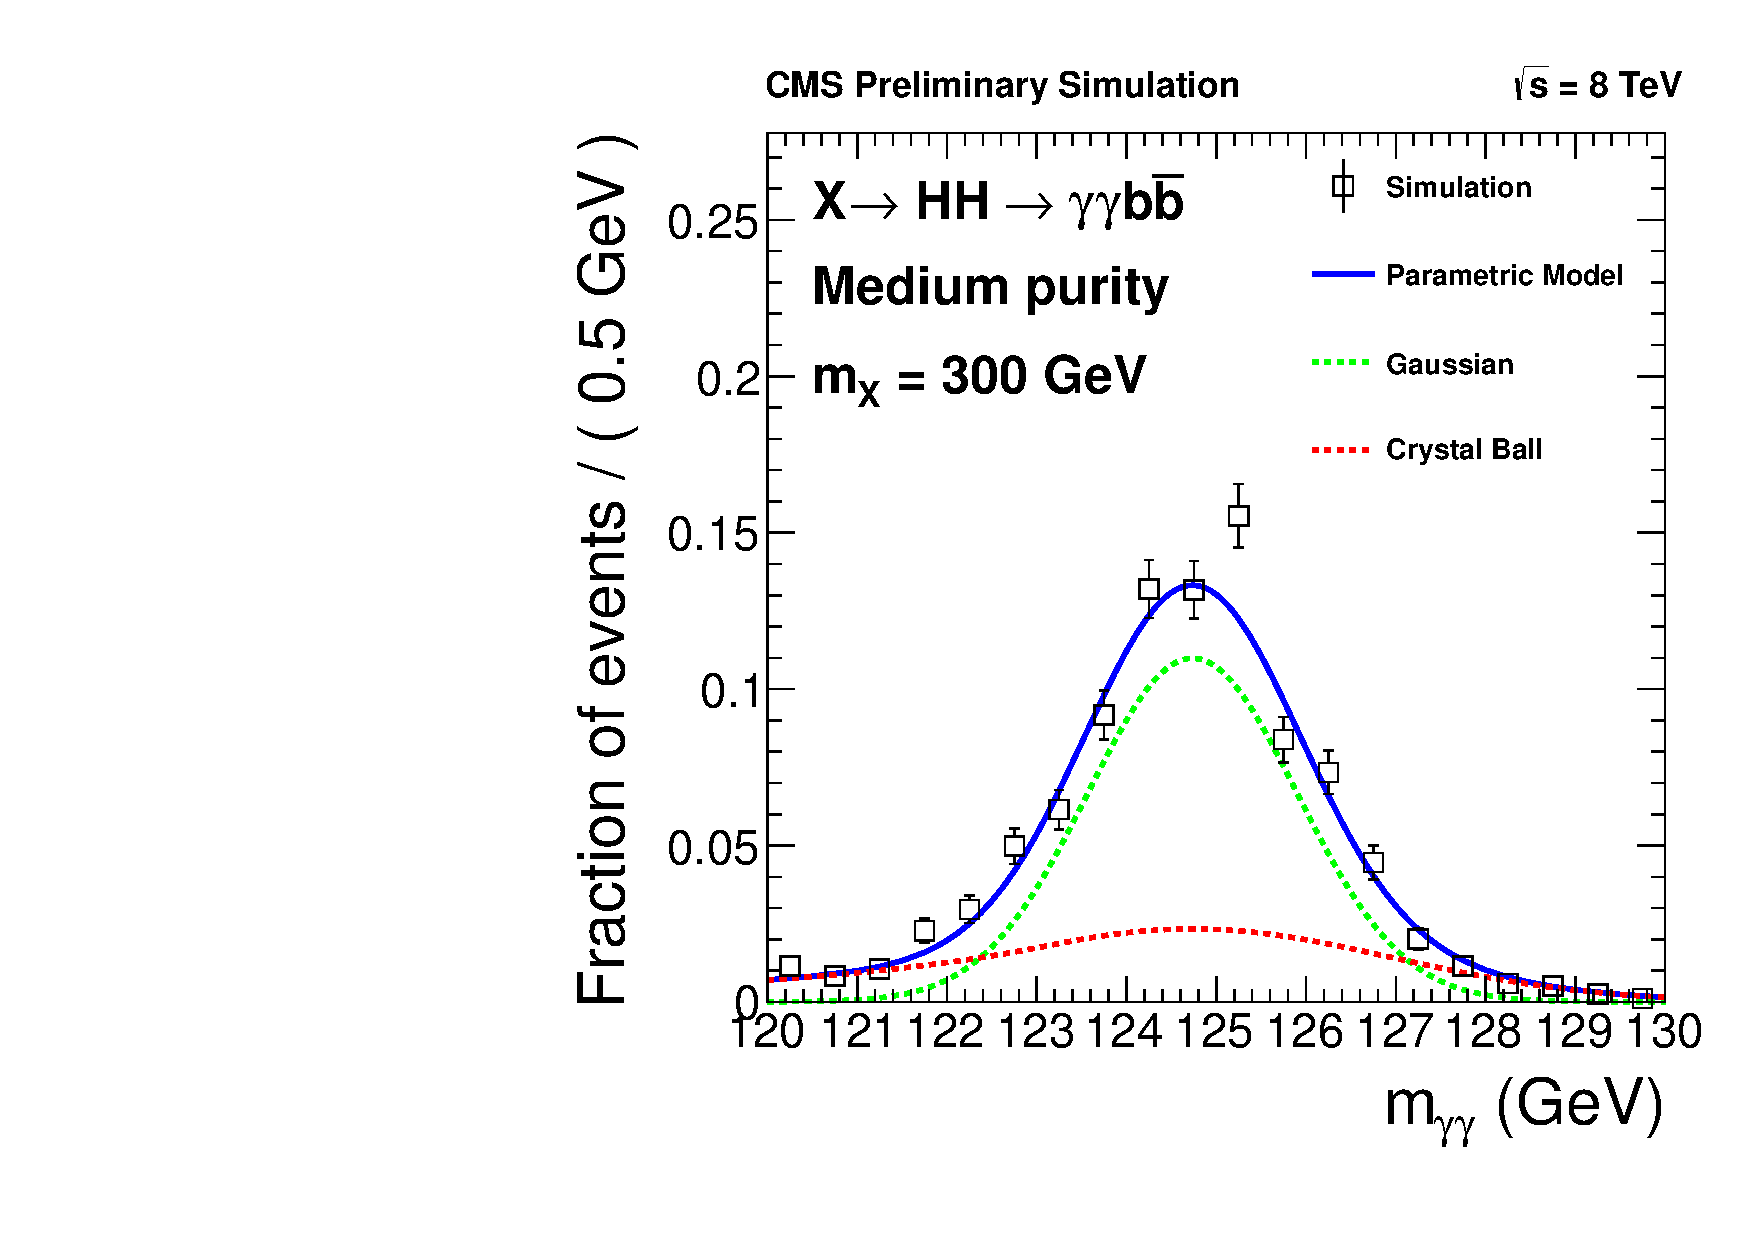
\includegraphics[width=0.70\textwidth]{figures/results/sigmodel_cat1_300.pdf}
 \end{center}
\caption{Simulated signal shape in the $\Mgg$ spectrum for the high-purity (top) and medium-purity
(bottom) categories for the Radion with mass 300 GeV. The open squares and corresponding
statistical uncertainties represent the simulation.
The blue line represents the model fitted to the simulation, while the green dashed line
and the red dashed line represent the two components of the model.}
\label{fig:sigfit_300}
\end{figure}

The background estimation is done by fitting the same distribution in each category on the interval
$[100, 180]$~GeV. This procedure is completely data-driven procedure, and as such it is important
that the choice of the function does not bias in a non-negligible way the estimate of the signal
strength obtained from the model conbining signal and background components.
The bias is estimated by considering a set of truth models which approximately describe the background.
For each truth model a large set of pseudo-data is generated and fitted by the sum of a candidate
background model and the signal model. The bias is defined as the ratio of the extracted signal strength
$\mu$ divided by the associated statistical uncertainty $\sigma_\mu$.
The bias is considered negligible if
\begin{equation}
\left|\text{median}\left(\frac{\mu}{\sigma_\mu}\right)\right| < 14\% \,.
\end{equation}
For both categories, more than one unbiased function was identified. For the limit extraction,
a power law is used for both categories. Figures~\ref{fig:datafit_260} and \ref{fig:datafit_300}
shows these fits to the data for four mass hypotheses.

\begin{figure}[ht]
 \begin{center}
   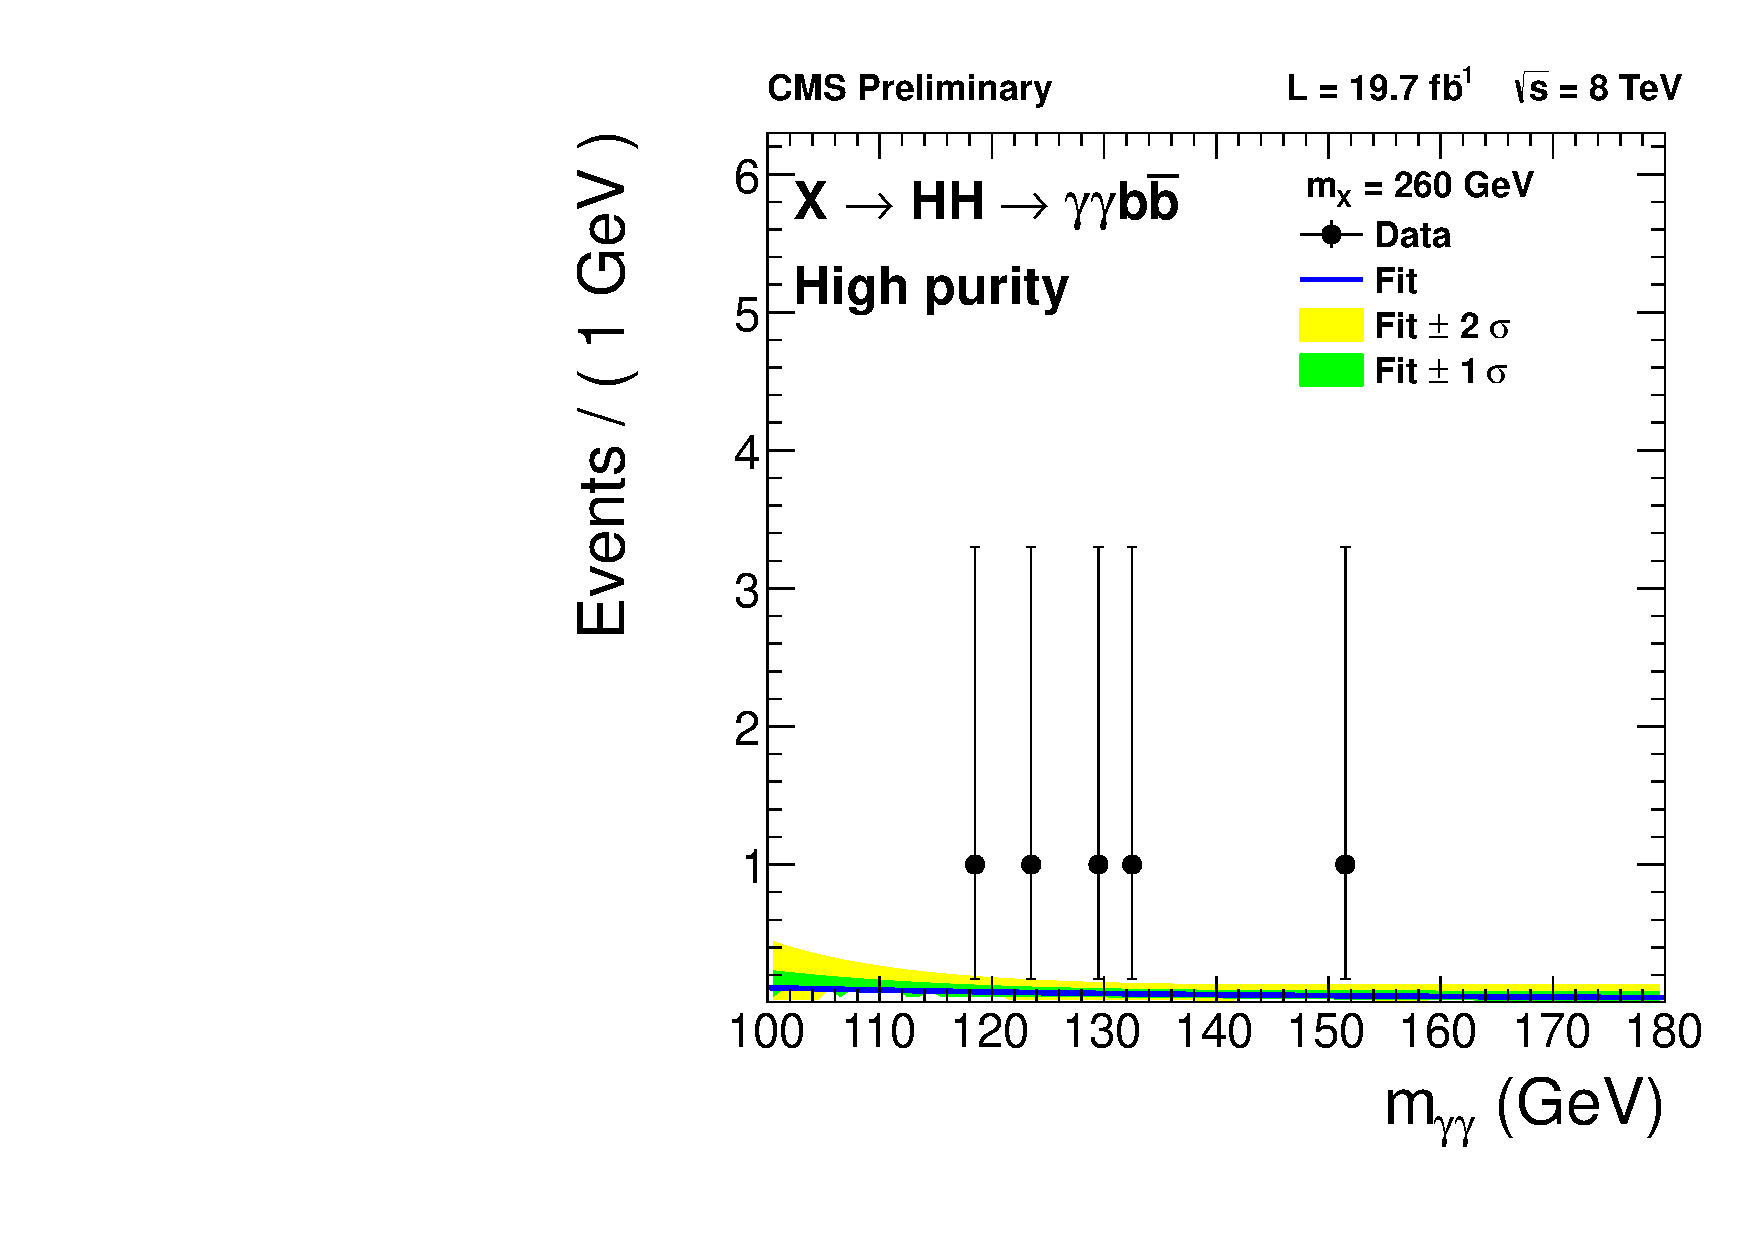
\includegraphics[width=0.45\textwidth]{figures/results/databkgoversig_cat0_260GeV.pdf}
   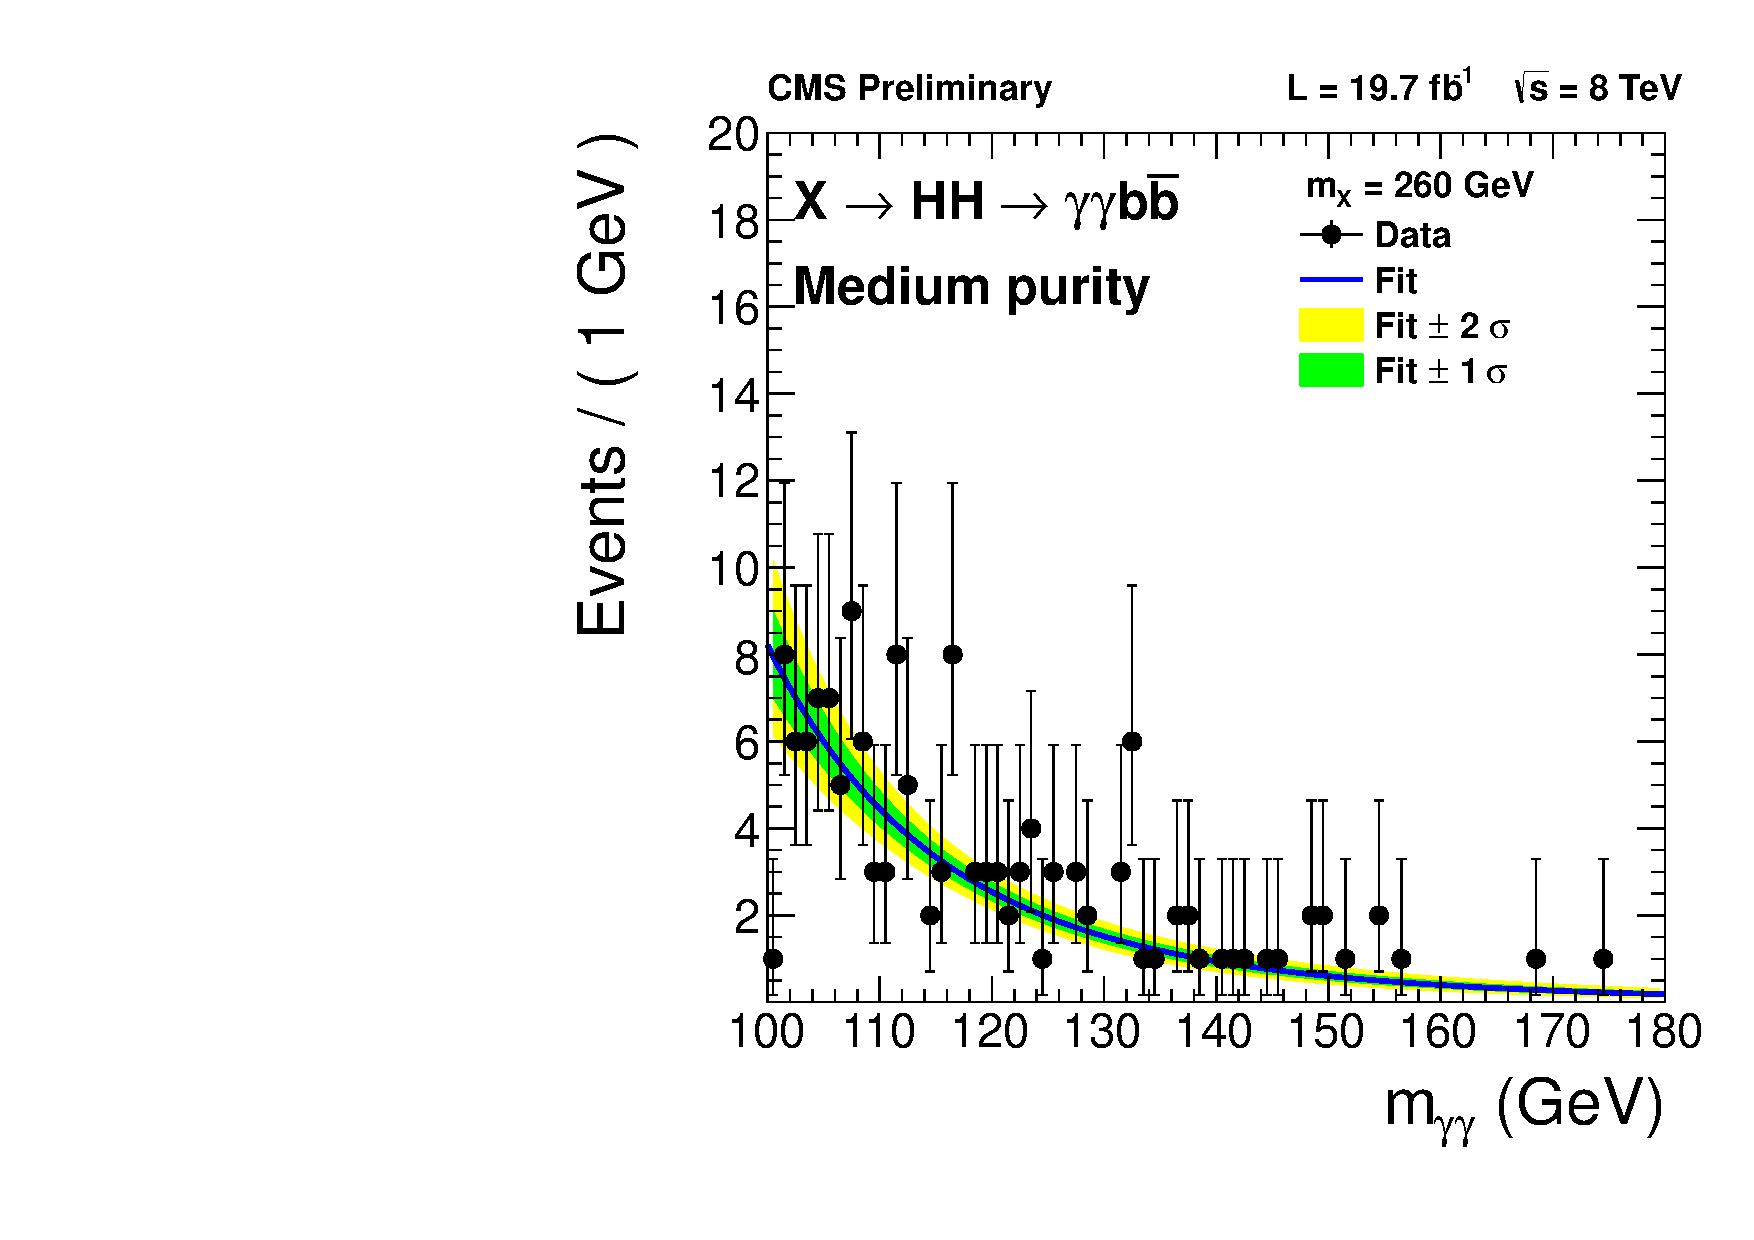
\includegraphics[width=0.45\textwidth]{figures/results/databkgoversig_cat1_260GeV.pdf}
   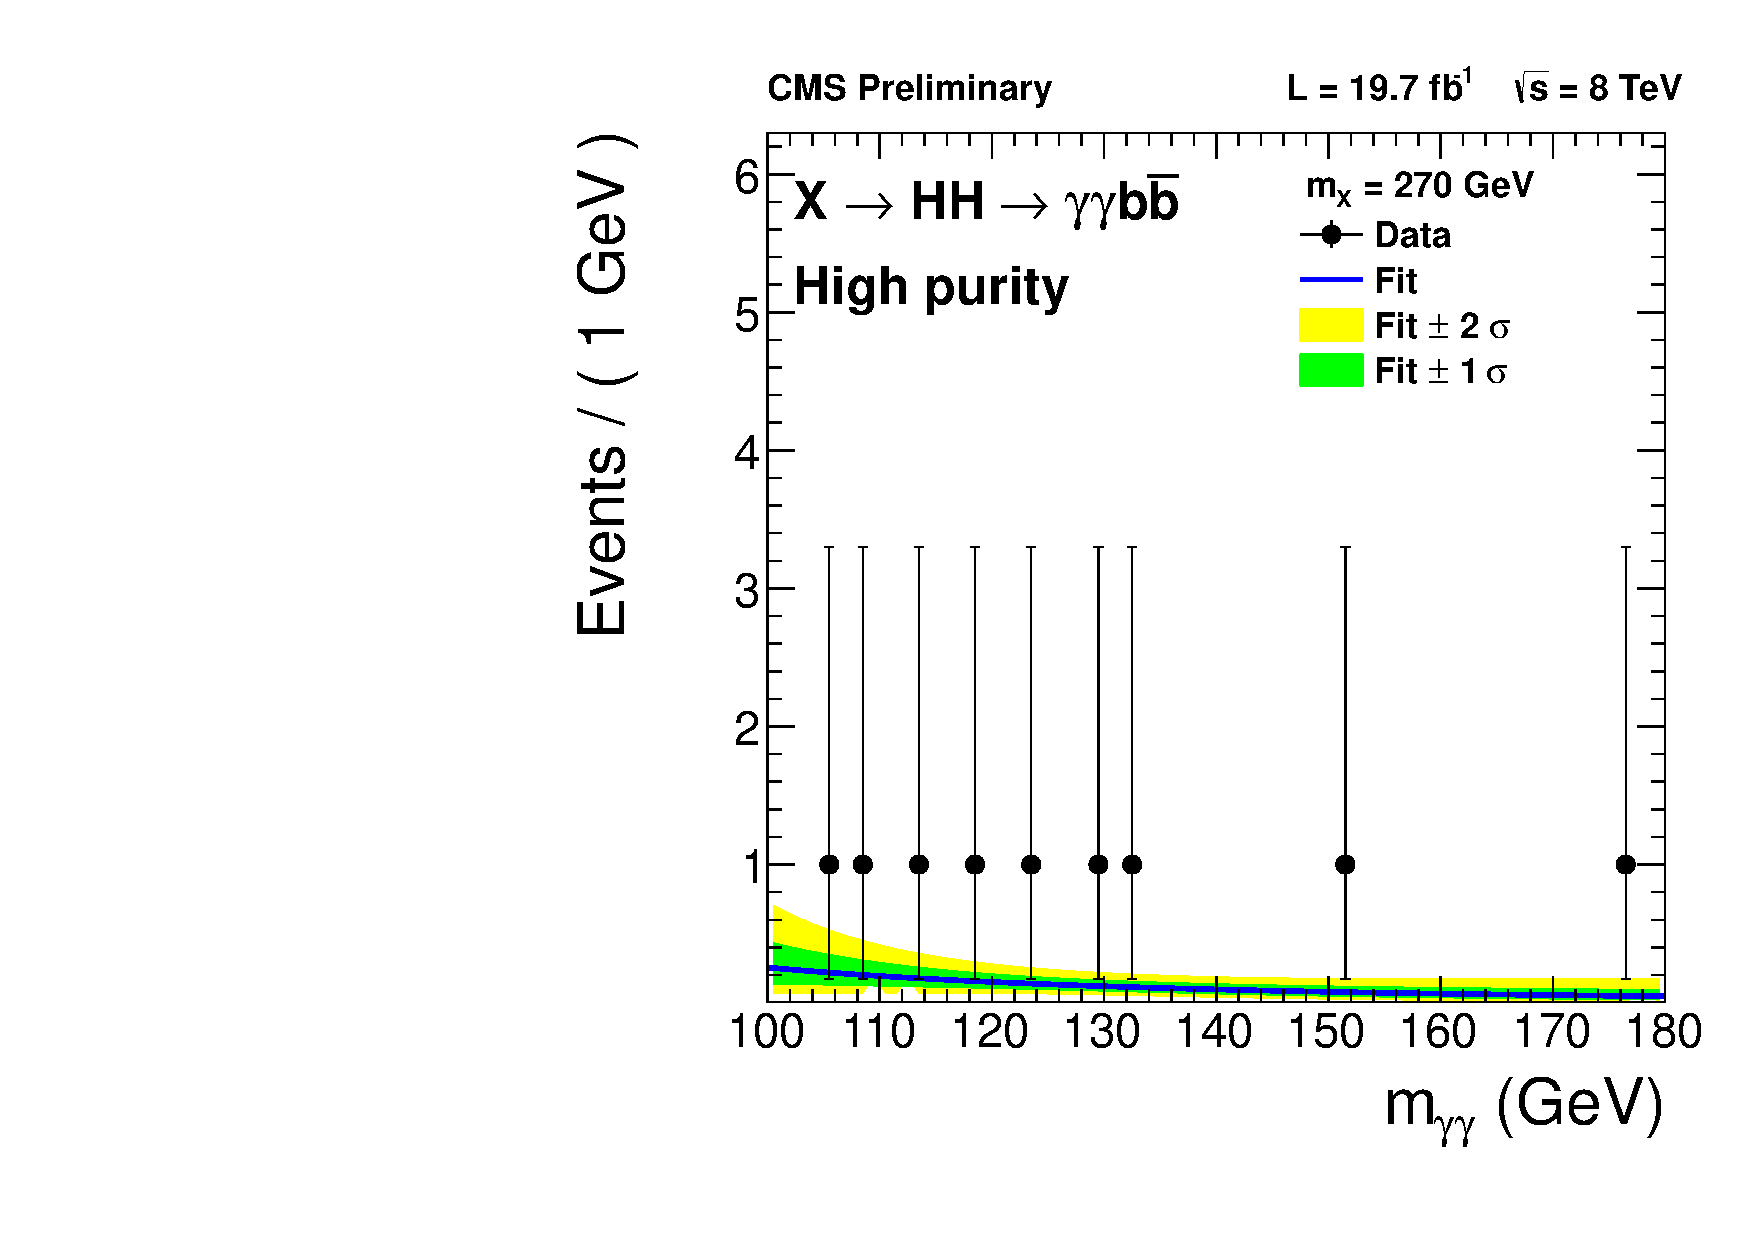
\includegraphics[width=0.45\textwidth]{figures/results/databkgoversig_cat0_270GeV.pdf}
   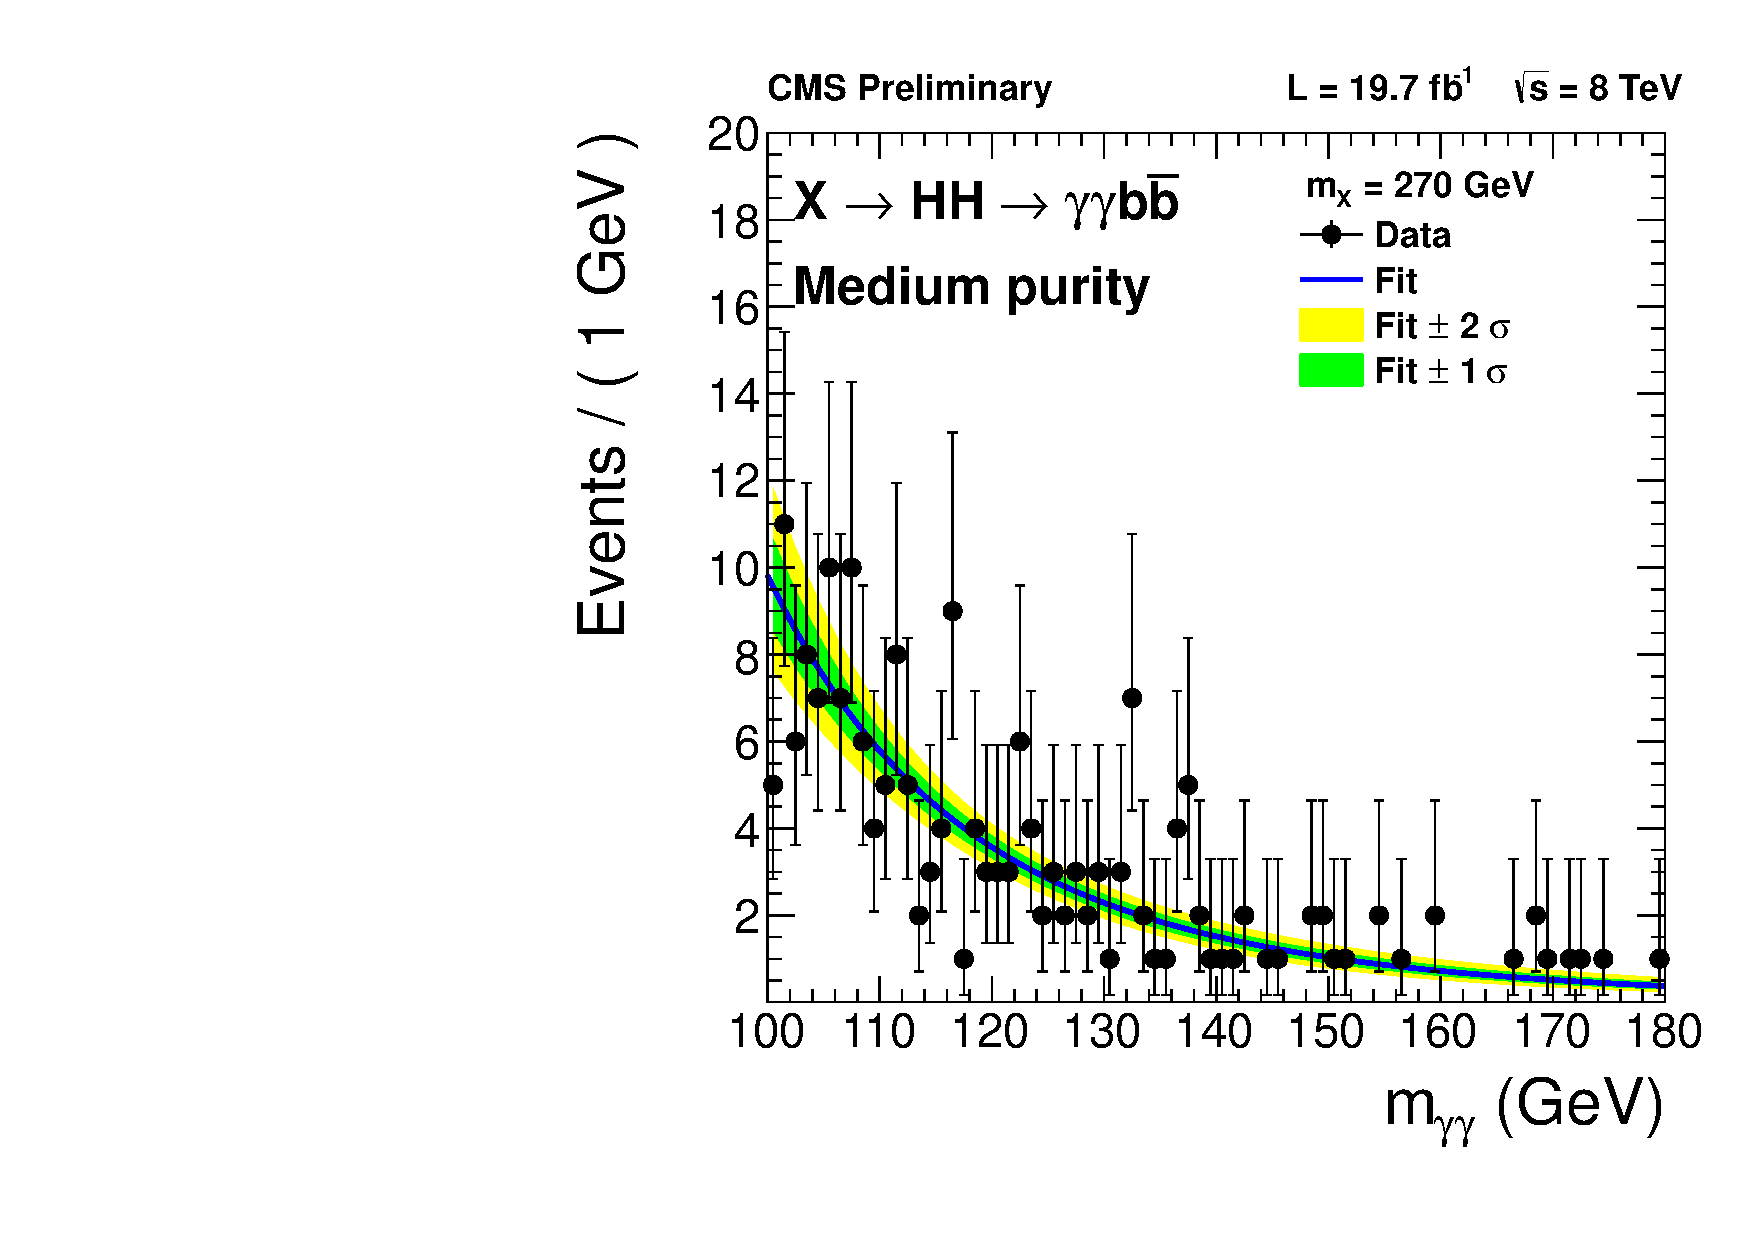
\includegraphics[width=0.45\textwidth]{figures/results/databkgoversig_cat1_270GeV.pdf}
 \end{center}
\caption{Events in the $\Mgg$ spectrum in the high-purity (left column) and medium-purity
(right column) categories for the resonance mass hypotheses 260 GeV (top row) and 270 GeV (bottom row).
The nonresonant component of the background is shown in blue
with 1$\sigma$ and 2$\sigma$ bands on the background estimation.}
\label{fig:datafit_260}
\end{figure}

\begin{figure}[ht]
 \begin{center}
   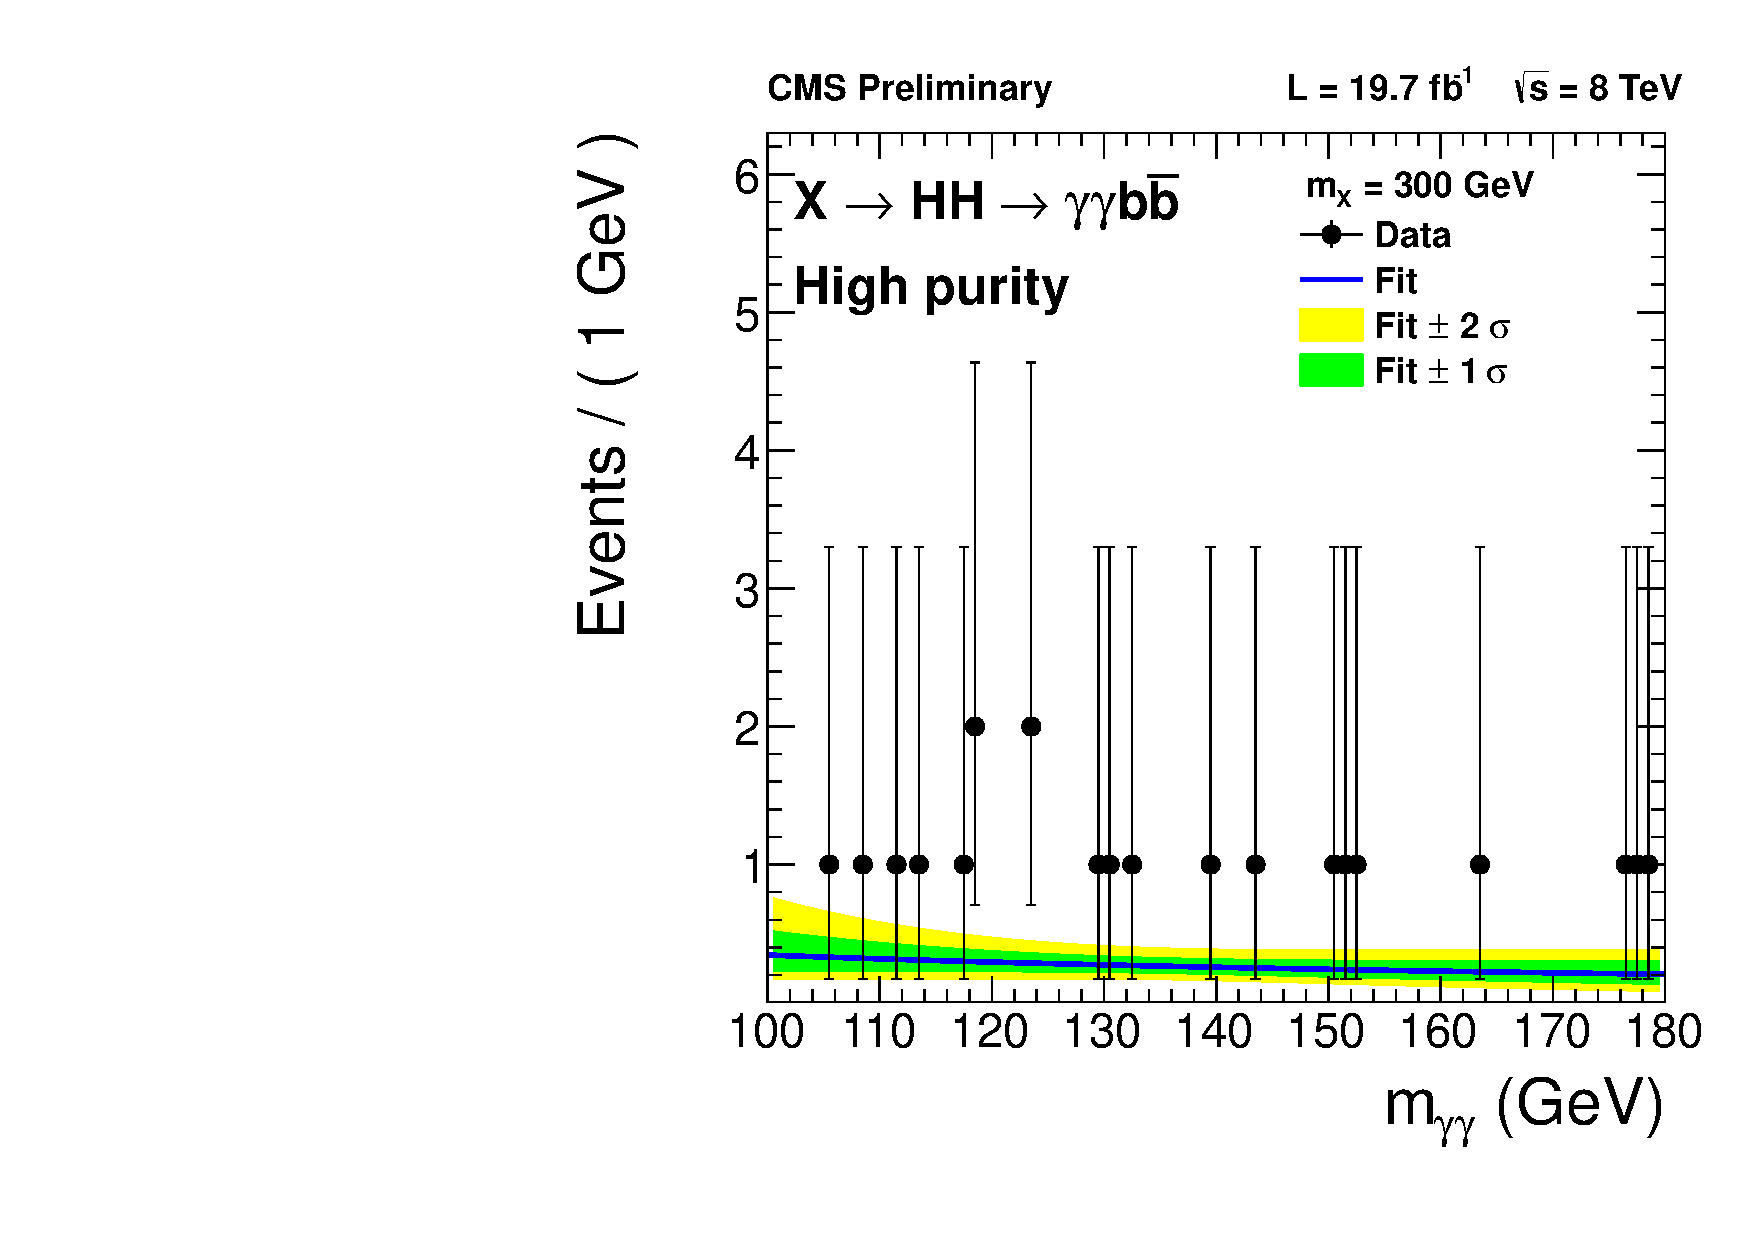
\includegraphics[width=0.45\textwidth]{figures/results/databkgoversig_cat0_300GeV.pdf}
   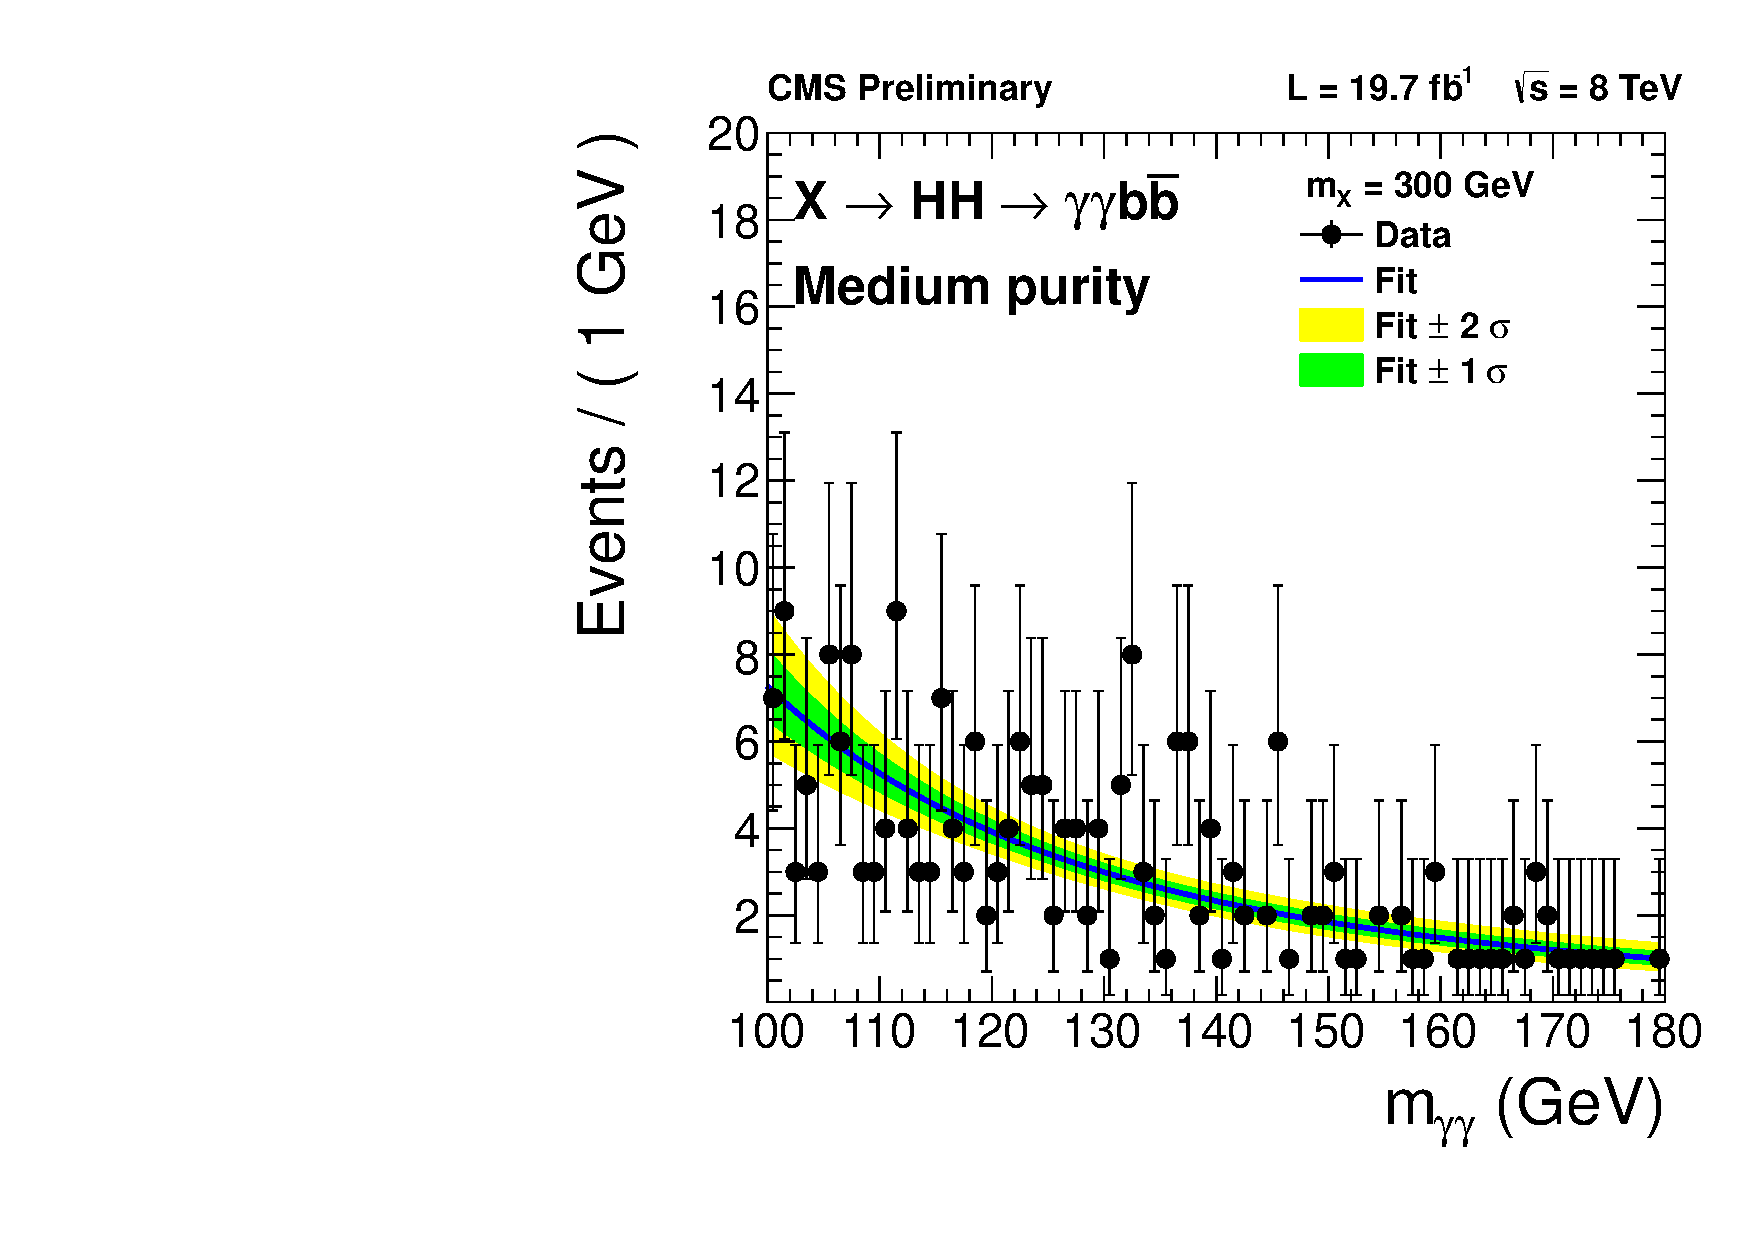
\includegraphics[width=0.45\textwidth]{figures/results/databkgoversig_cat1_300GeV.pdf}
   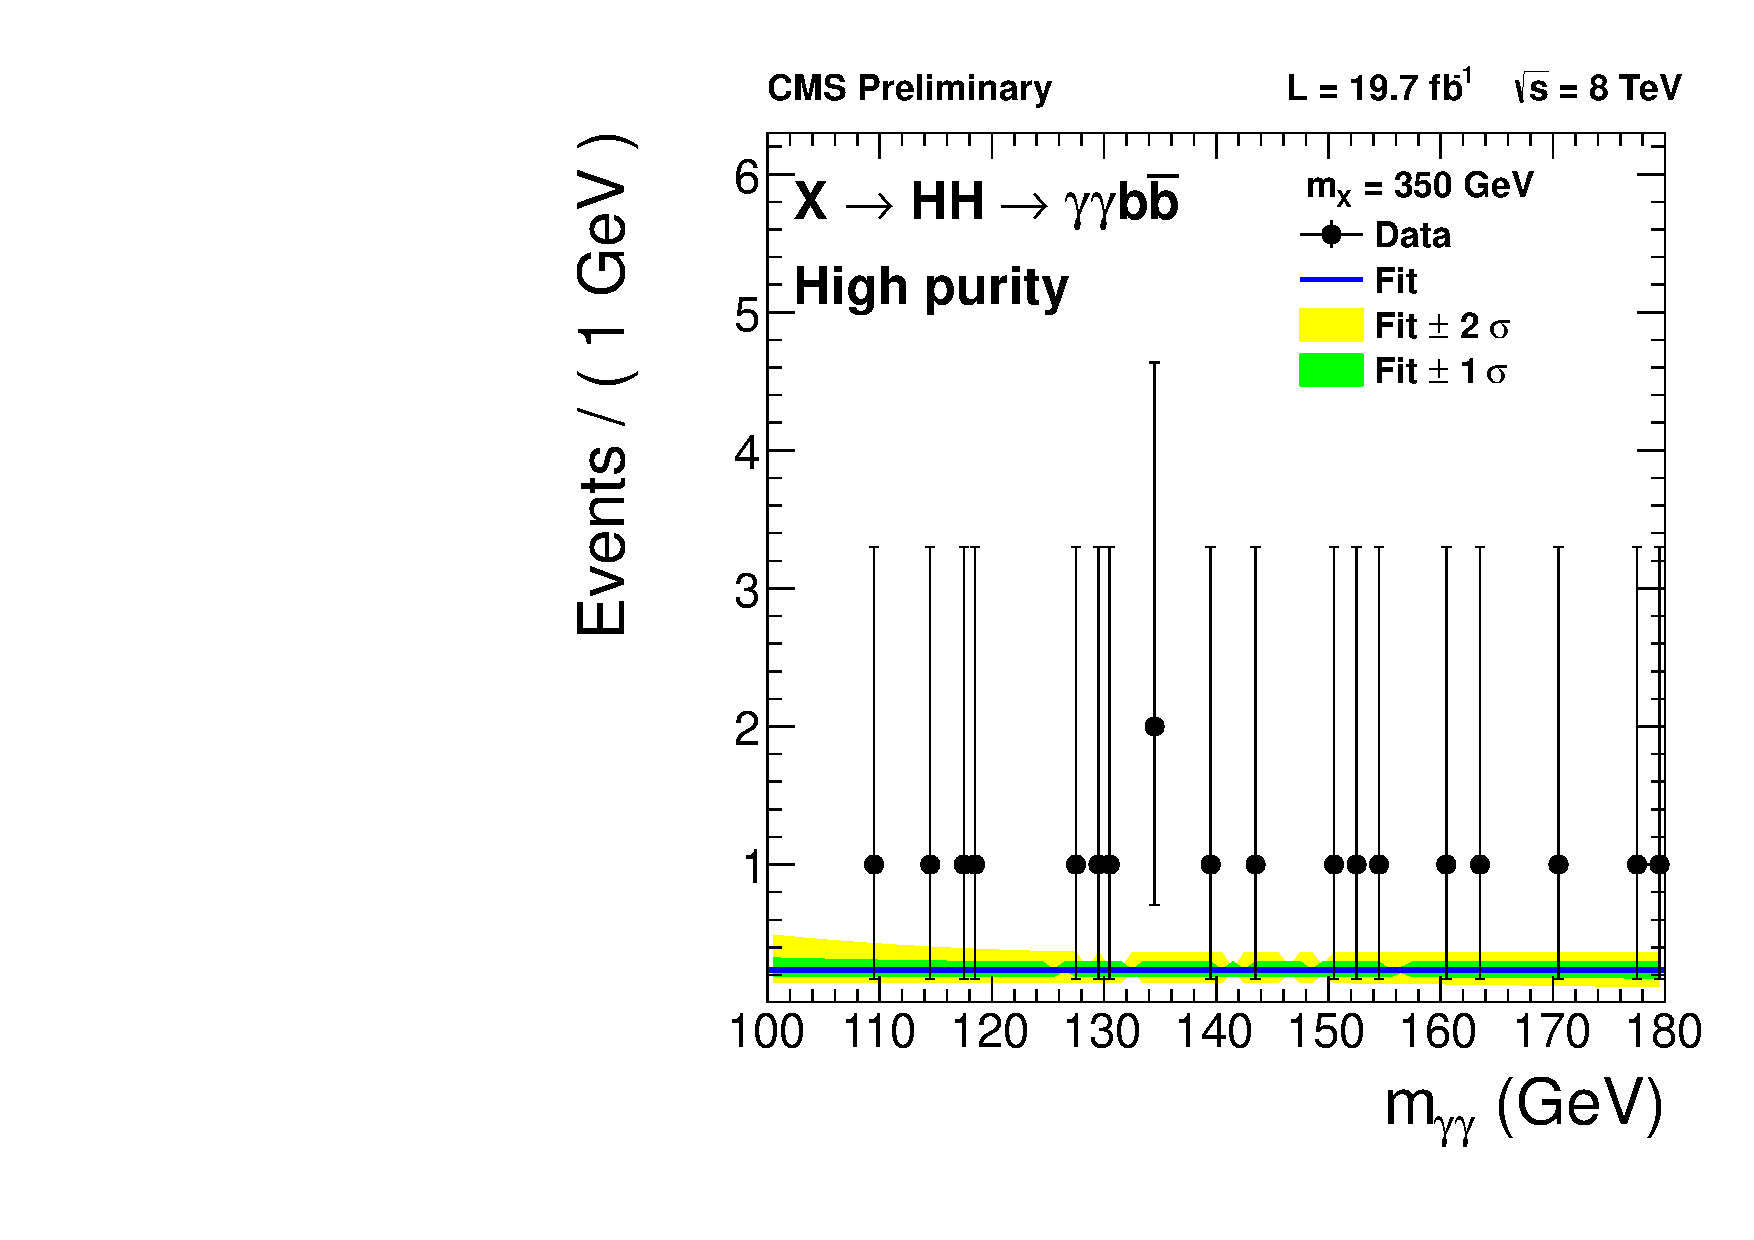
\includegraphics[width=0.45\textwidth]{figures/results/databkgoversig_cat0_350GeV.pdf}
   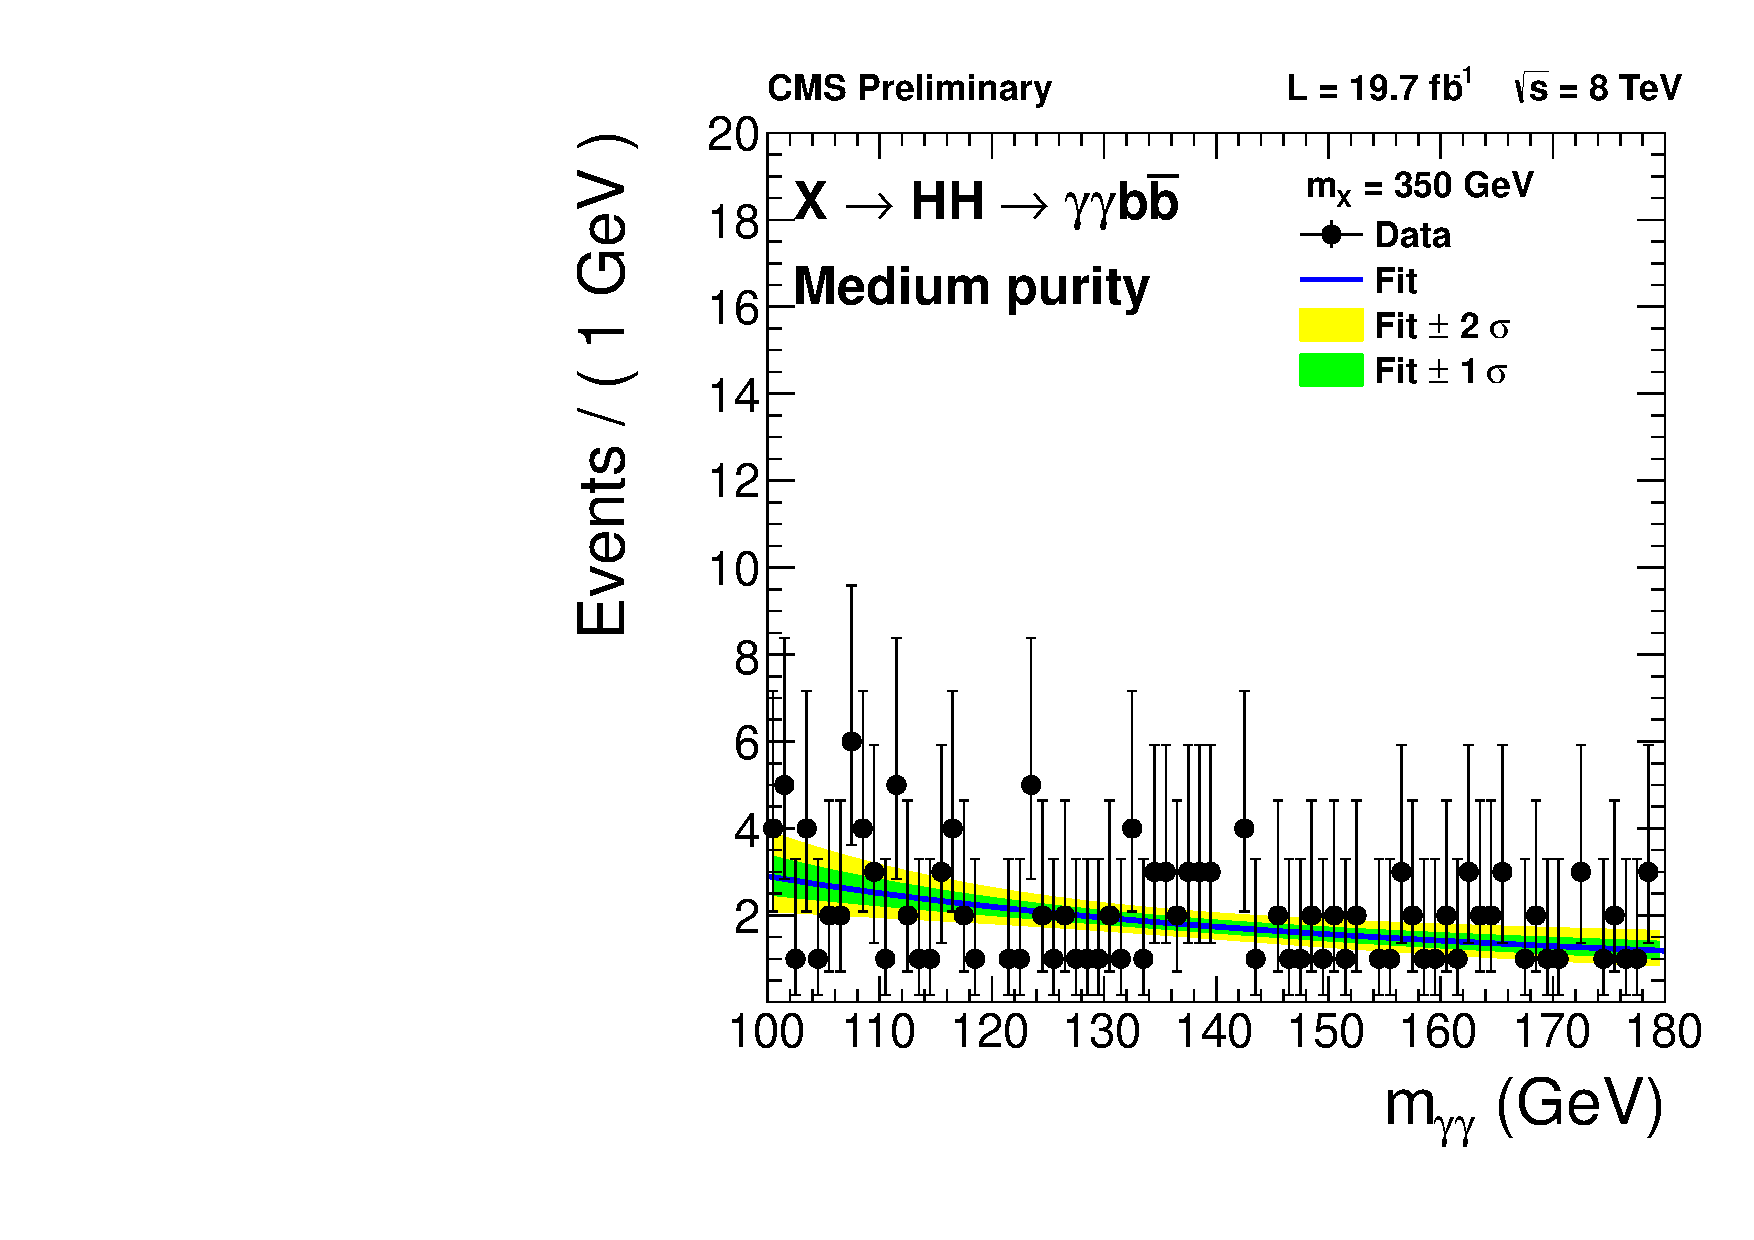
\includegraphics[width=0.45\textwidth]{figures/results/databkgoversig_cat1_350GeV.pdf}
 \end{center}
\caption{Events in the $\Mgg$ spectrum in the high-purity (left column) and medium-purity
(right column) categories for the resonance mass hypotheses 300 GeV (top row) and 350 GeV (bottom row)
The nonresonant component of the background is shown in blue
with 1$\sigma$ and 2$\sigma$ bands on the background estimation.}
\label{fig:datafit_300}
\end{figure}

The background fit estimates only the nonresonant contribution arising from diphoton
production. The contribution from SM Higgs production with $\Hgg$ could create a peak in the
spectrum that mimics the signal process. This resonant background
contribution is therefore added in the fit and accounted for in the limits.
The expected contribution of the resonant background is small, and the
effect on the final result is found to be at most 2\%.

There is no excess above the expectation observed, so the analysis proceeds to calculating
upper limits on the signal cross section.
The 95\% CL for expected and observed median upper limits is shown in
Table~\ref{table:limits_lowmass} and Figure~\ref{fig:limits_lowmassres}
for both categories and for the high-purity category only.
The latter result is provided to simplify the comparison with new physics models where
the Higgs branching ratios for the $\Hgg$ and $\Hbb$ decays can be modified from the SM.
The green and yellow bands represent the 1$\sigma$ and 2$\sigma$
confidence intervals around the expected limit. Theory expectations for Radion, RS1 KK-graviton, and 
bulk KK-graviton are shown, where the Radion expectation assumes $\text{BR}(R\rightarrow HH) =$~25\%
for all Radion masses above 300 GeV. Through comparison with the Graviton simulation,
the search is verified to be spin-independent, so theory expectations for both spin-0 and spin-2
hypotheses may be overlaid together.

\begin{table}[ht]
  \centering
  \renewcommand{\arraystretch}{1.4}
  \caption{Observed and median expected 95\% CL upper limits for $m_X \le 400$~GeV.}
  \begin{tabular}{ | c || c | c || c | c |}
\hline
$m_X$ (GeV) & Observed limit (fb) & Expected limit (fb) & Observed limit (fb) & Expected limit (fb) \\ \hline
 & & &  \multicolumn{2}{c|}{High-purity category only} \\ \hline
260 & 3.14 & 2.12 & 3.54 & 2.41 \\
270 & 2.70 & 2.40 & 3.07 & 2.74 \\
300 & 3.98 & 2.73 & 3.64 & 3.14 \\
350 & 1.67 & 2.23 & 2.17 & 2.66 \\
400 & 1.97 & 1.66 & 3.40 & 2.01 \\ \hline
\end{tabular}

  \label{table:limits_lowmass}
\end{table}

\begin{figure}[ht]
 \begin{center}
   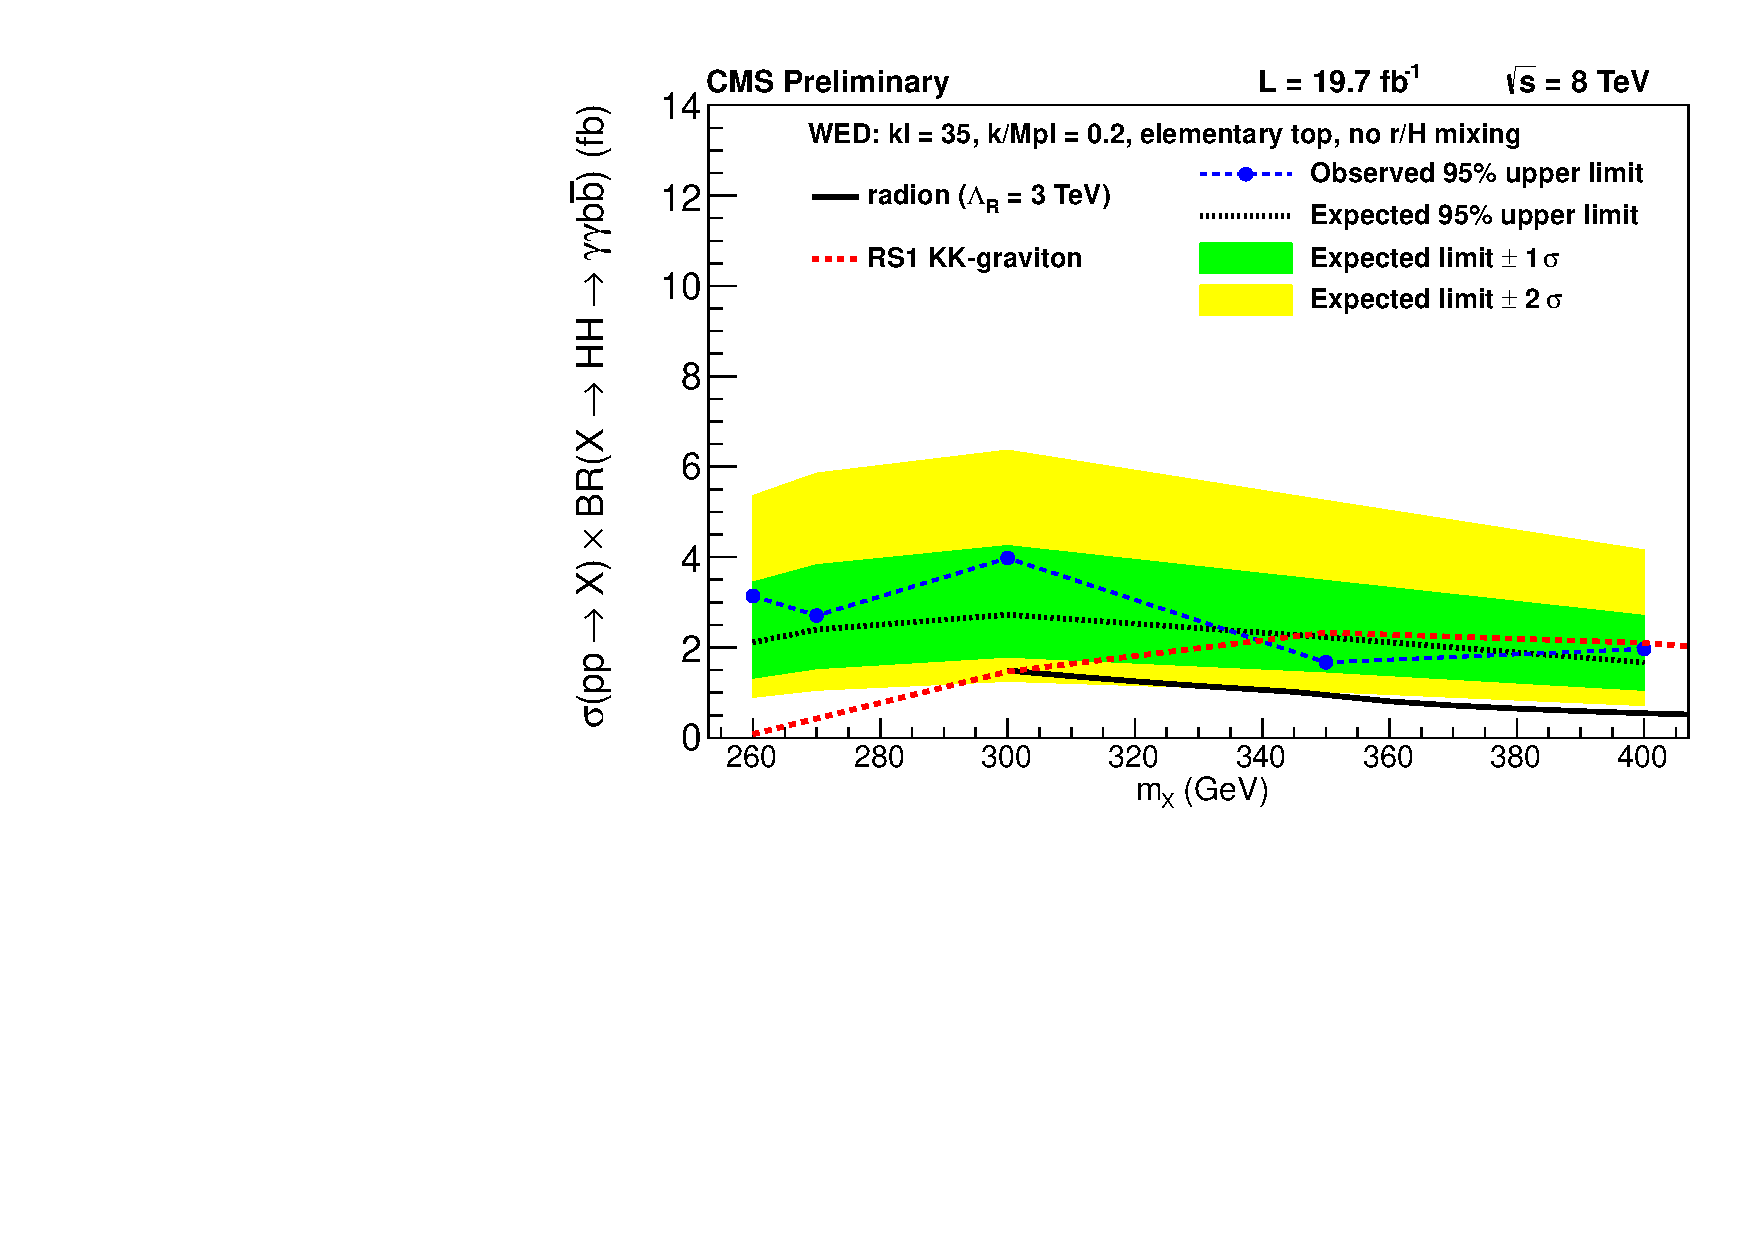
\includegraphics[width=0.7\textwidth]{figures/results/WP4_cutbased_low_all.pdf}
   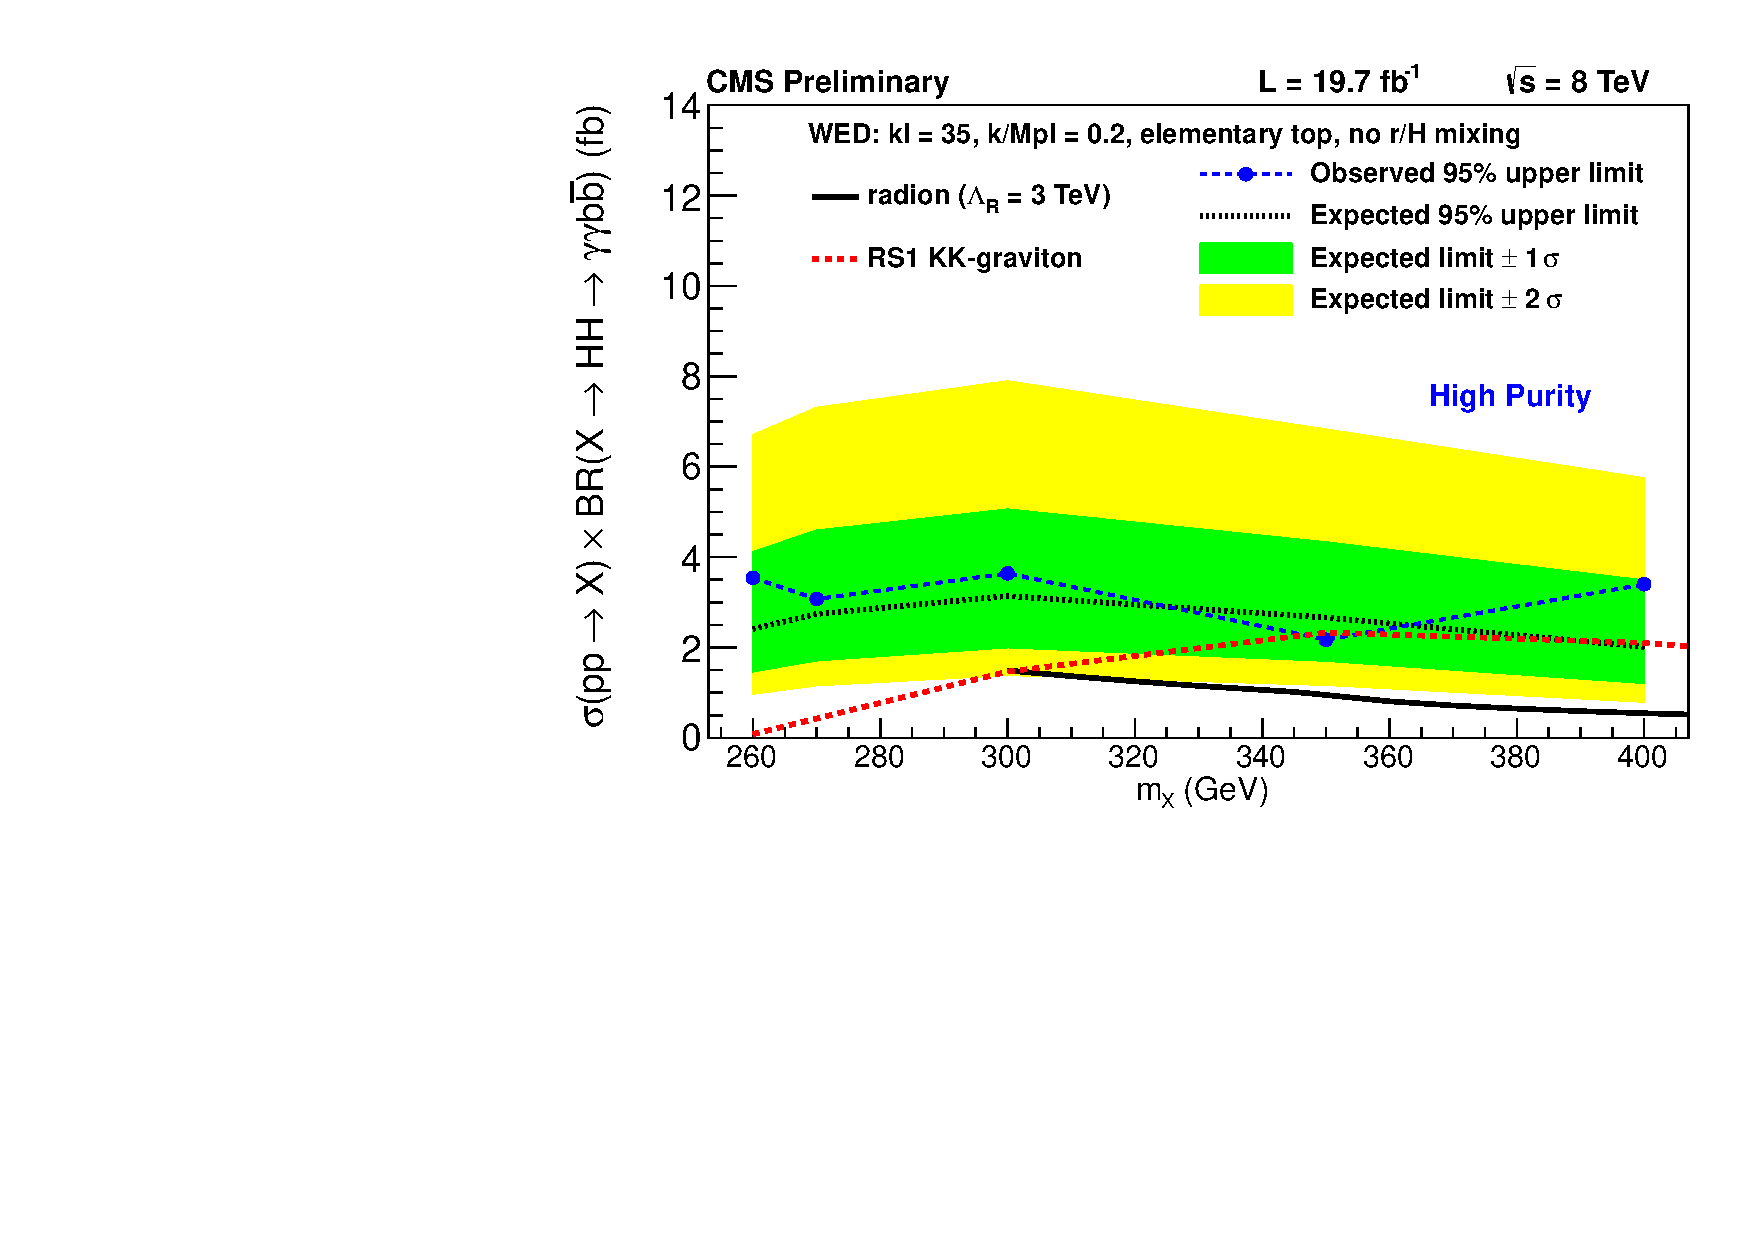
\includegraphics[width=0.7\textwidth]{figures/results/WP4_cutbased_low_base_onecat.pdf}
 \end{center}
\caption{Expected 95\% CL upper limits on the cross section times branching ratios
$\sigma(pp\rightarrow X) \times \text{BR}( X \rightarrow HH \rightarrow \gamma\gamma b\bar{b})$.
Theory lines corresponding to WED models with Radion, RS1 KK-graviton, and bulk KK-graviton are
overlaid. Limits from both categories (top) and high-purity category only (bottom) are shown.
The results are obtained using the asymptotic $\text{CL}_s$ approach.}
\label{fig:limits_lowmassres}
\end{figure}

\subsection{High-mass Resonant Results}

For the high-mass resonant search, the signal yield is extracted by fitting the $\Mggjjk$ spectrum.
in a procedure similar to the one for the low-mass resonant search. The signal model is built
for each mass hypothesis by fitting the $\Mggjjk$ peak in the simulation sample separately for the
two categories. The functional form used is the sum of a Crystal Ball and Gaussian with the means
constrained to be the same. The position of the peak follows the closely the respective $m_X$
hypothesis,
and the resolution in the peak improves as $m_X$ increases. Figure~\ref{fig:sigfit_500_1000}
shows examples of the signal fit for mass hypotheses of 500 GeV and 1 TeV.

\begin{figure}[ht]
 \begin{center}
   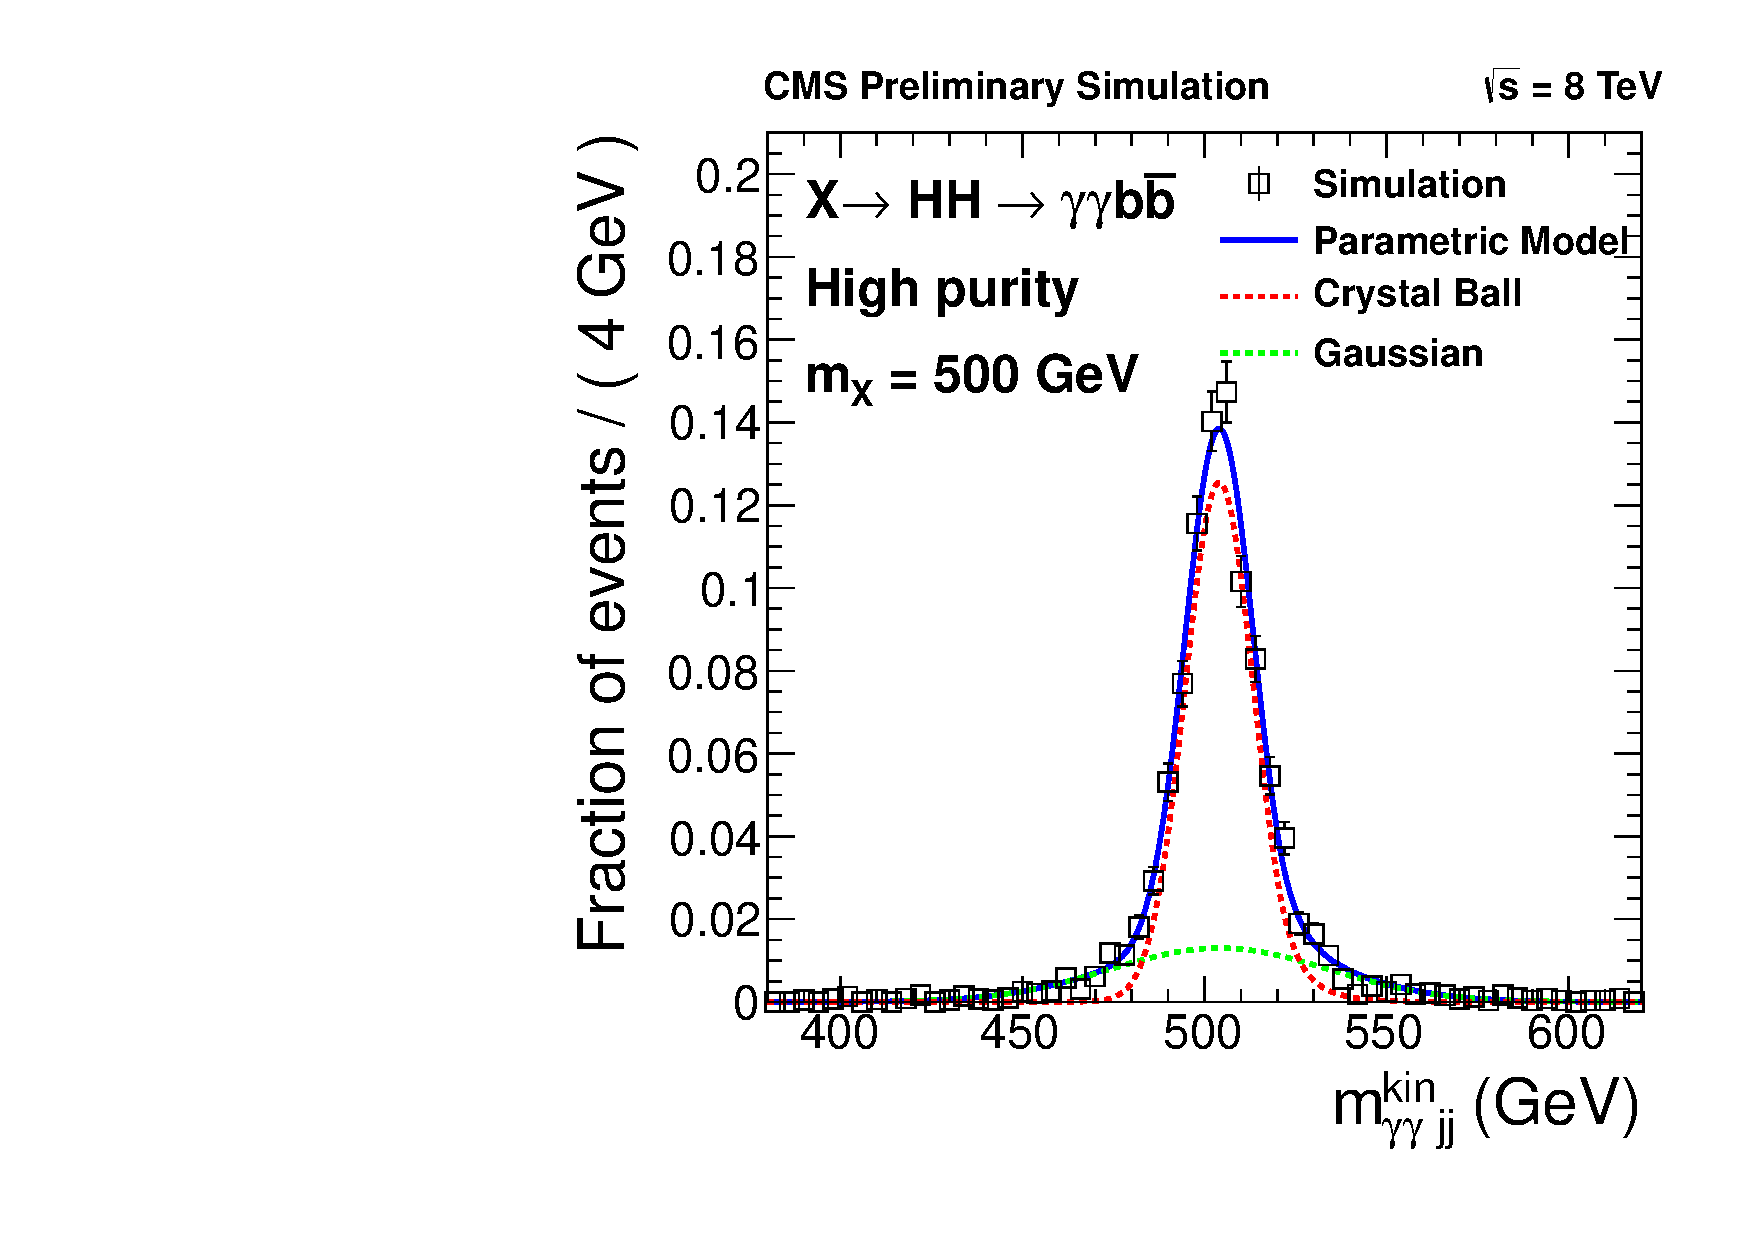
\includegraphics[width=0.45\textwidth]{figures/results/sigmodel_cat0_500GeV.pdf}
   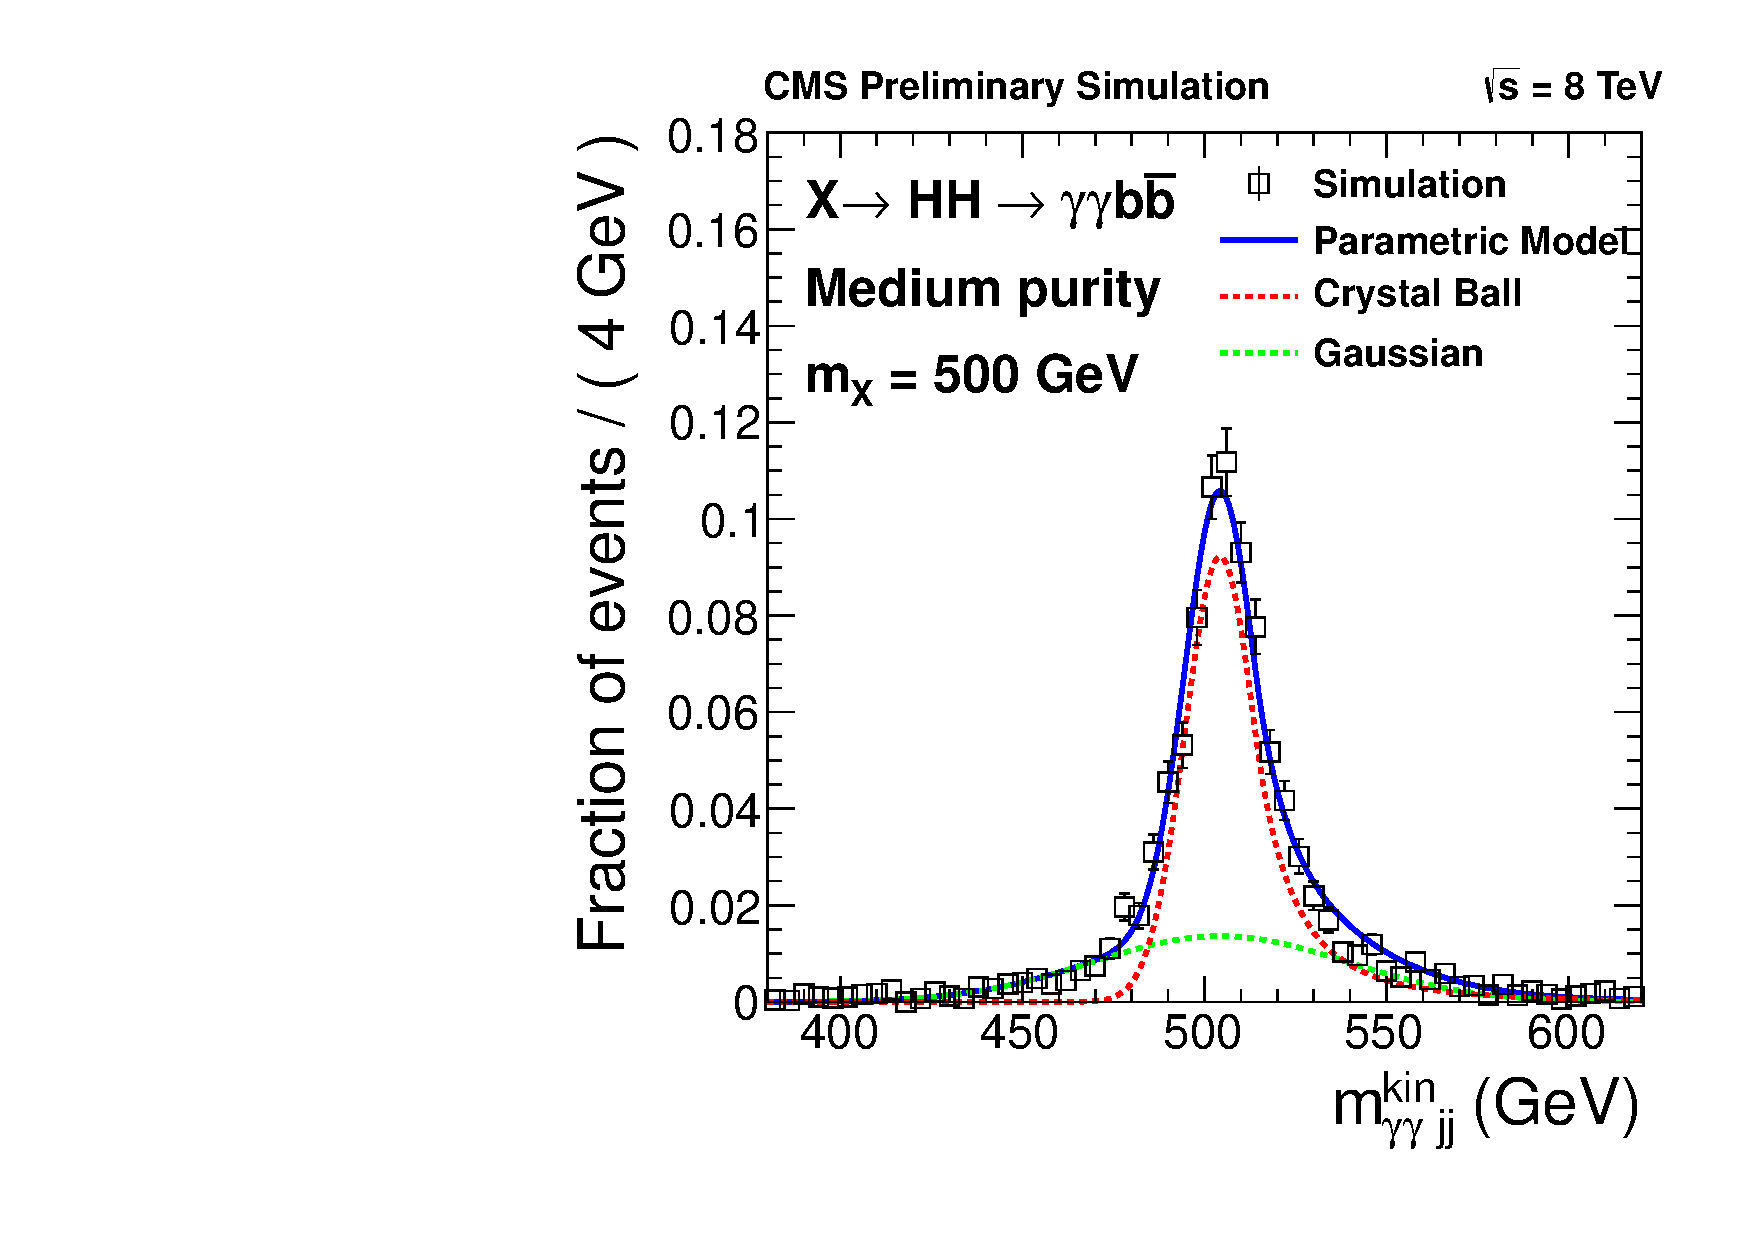
\includegraphics[width=0.45\textwidth]{figures/results/sigmodel_cat1_500GeV.pdf}
   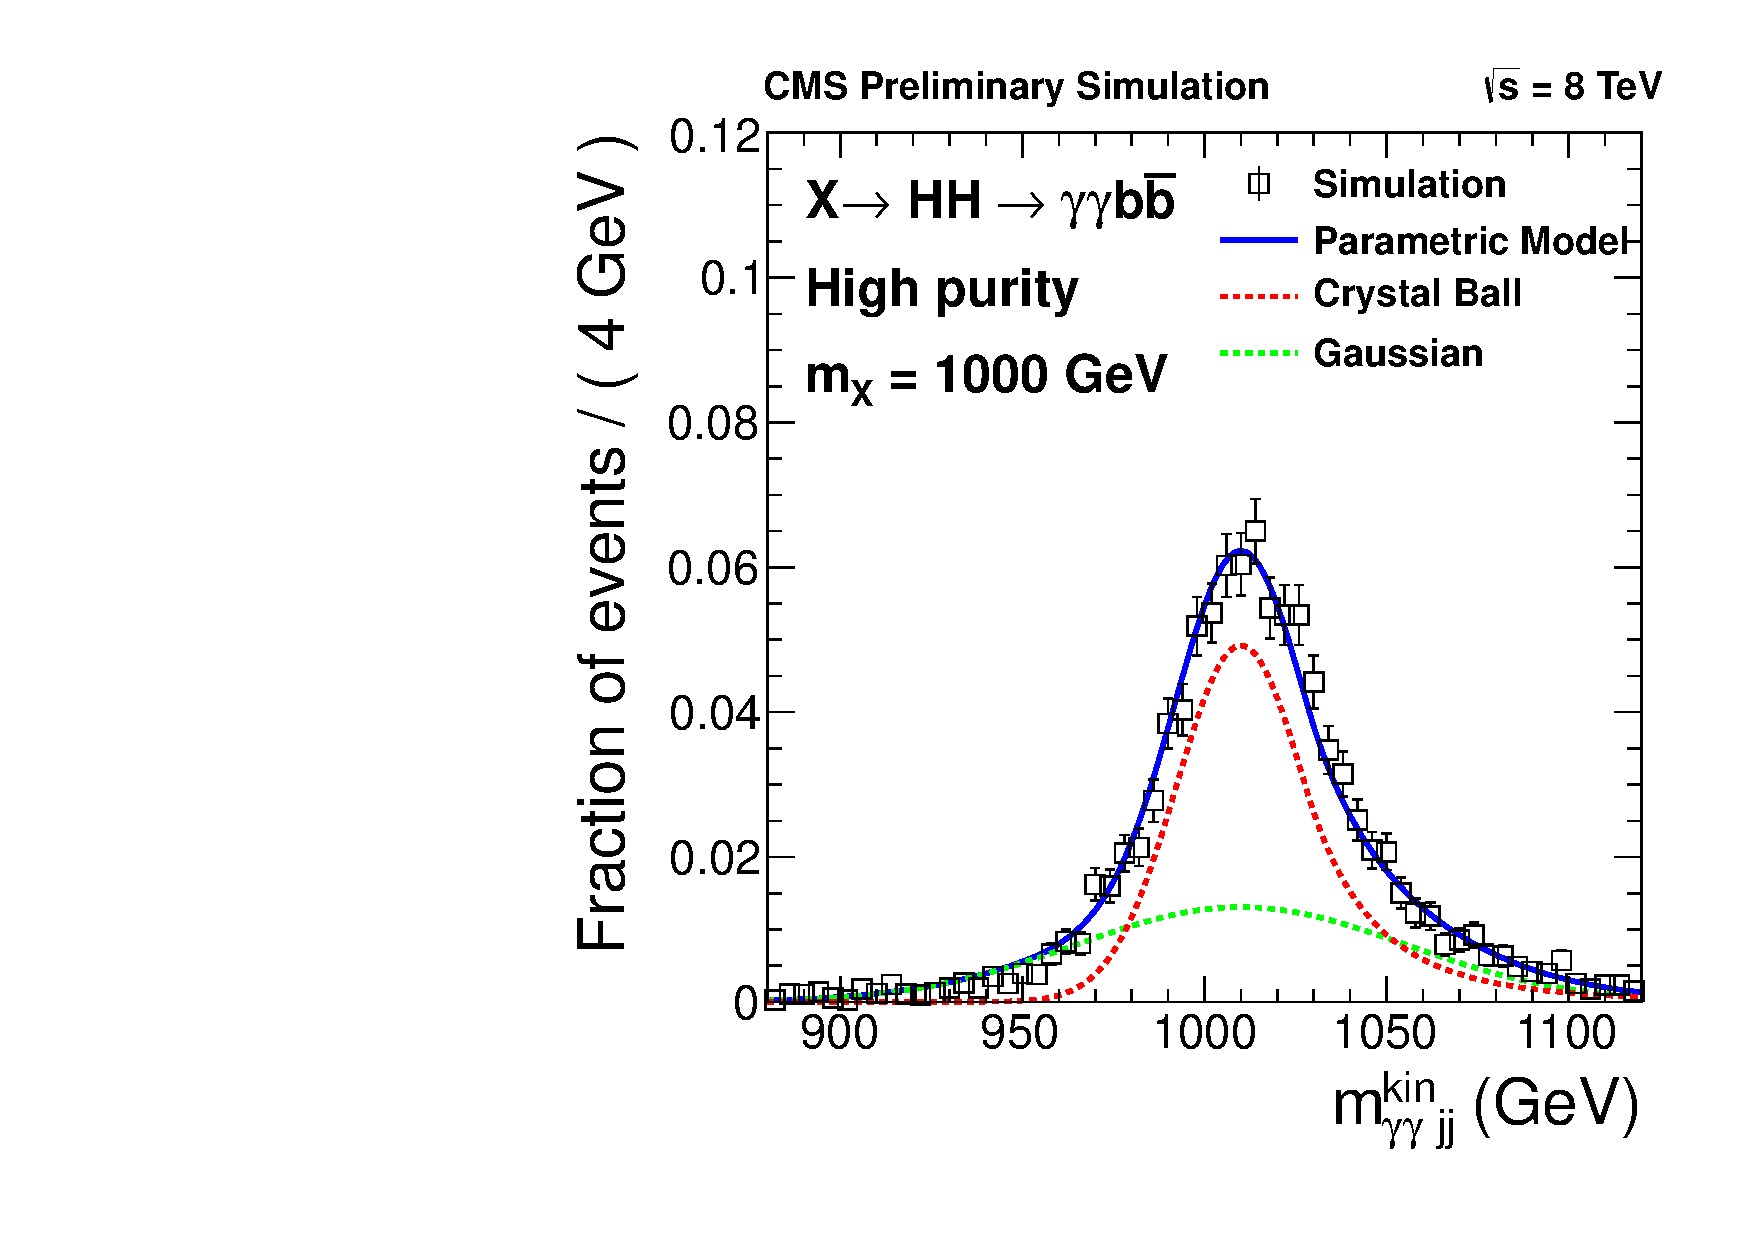
\includegraphics[width=0.45\textwidth]{figures/results/sigmodel_cat0_1000GeV.pdf}
   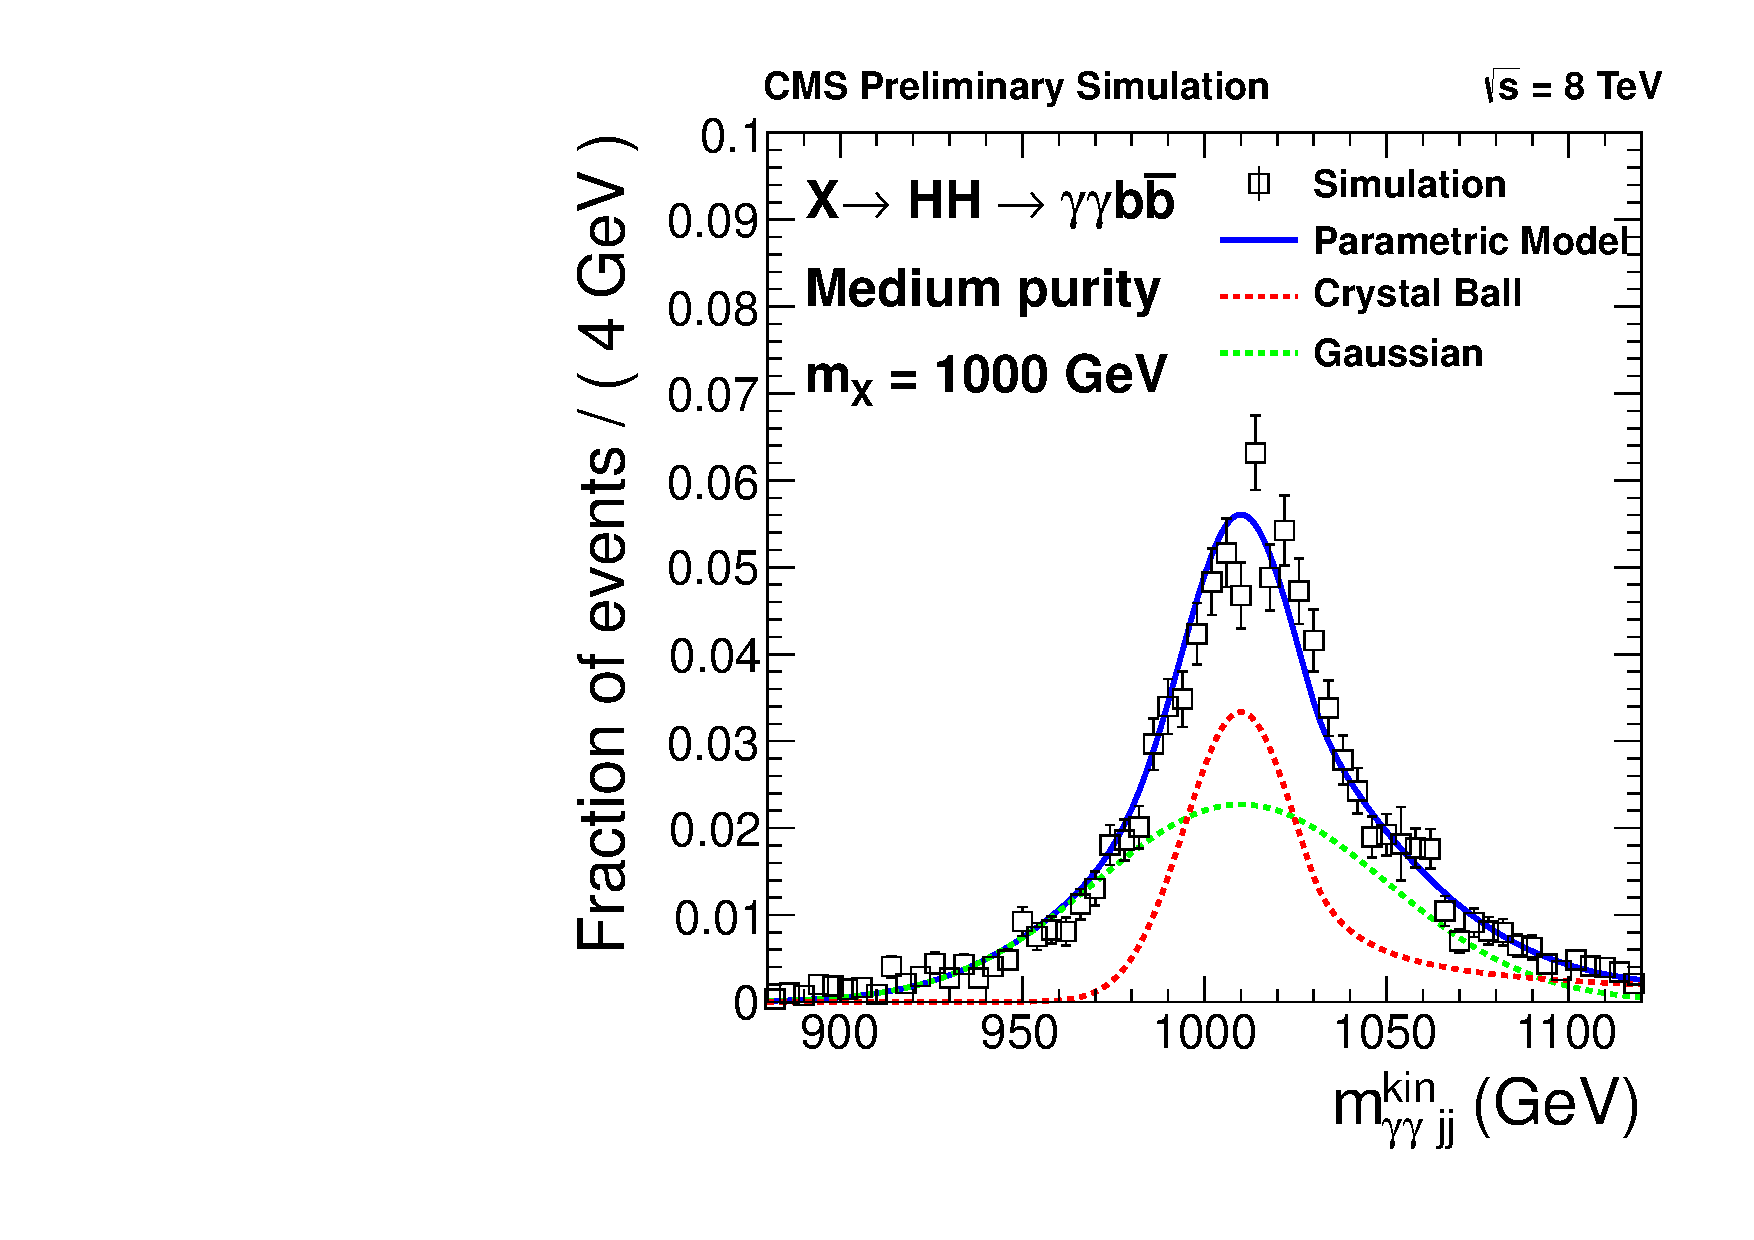
\includegraphics[width=0.45\textwidth]{figures/results/sigmodel_cat1_1000GeV.pdf}
 \end{center}
\caption{Simulated signal shape in the $\Mggjjk$ spectrum for the high-purity (left column)
and medium-purity (right column) categories for the Radion with mass 500 GeV (top row) and
1 TeV (bottom row). The open squares and corresponding
statistical uncertainties represent the simulation.
The blue line represents the model fitted to the simulation, while the green dashed line
and the red dashed line represent the two components of the model.}
\label{fig:sigfit_500_1000}
\end{figure}


The background estimation is done by fitting the same distribution in each category on the interval
$[320, 1200]$~GeV. The lower edge is chosen to avoid the kinematic turn-on of the background
while still ensuring full containment for the 400 GeV signal. The same bias estimation procedure
described for the low-mass resonant search is applied here. The chosen background function is a power
law for both categories, shown in Figure~\ref{fig:datafit_4body}. Note that in this regime,
the SM Higgs background does not have a resonance on the $\Mggjjk$ spectrum, so
there is no signal contamination from a background process.

\begin{figure}[ht]
 \begin{center}
   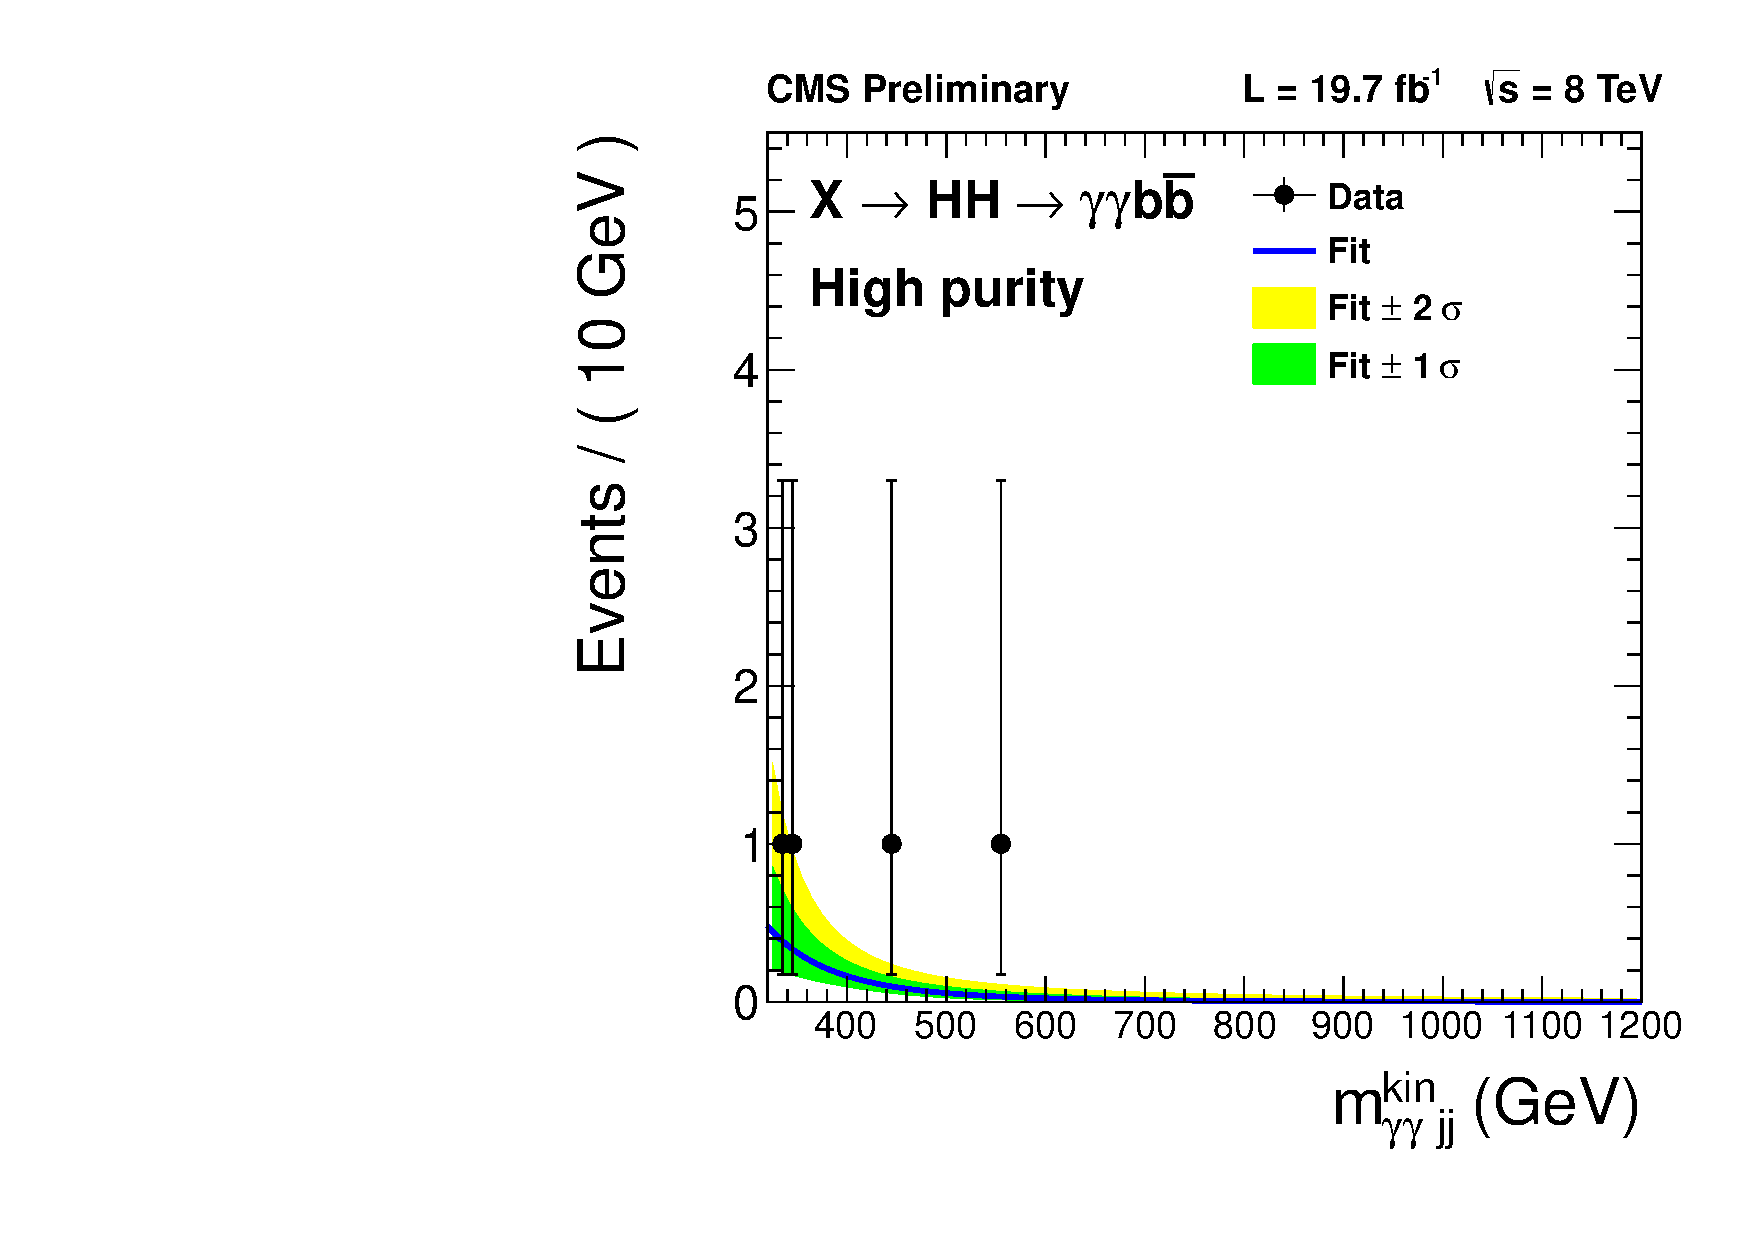
\includegraphics[width=0.70\textwidth]{figures/results/databkgoversig_cat0_4body.pdf}
   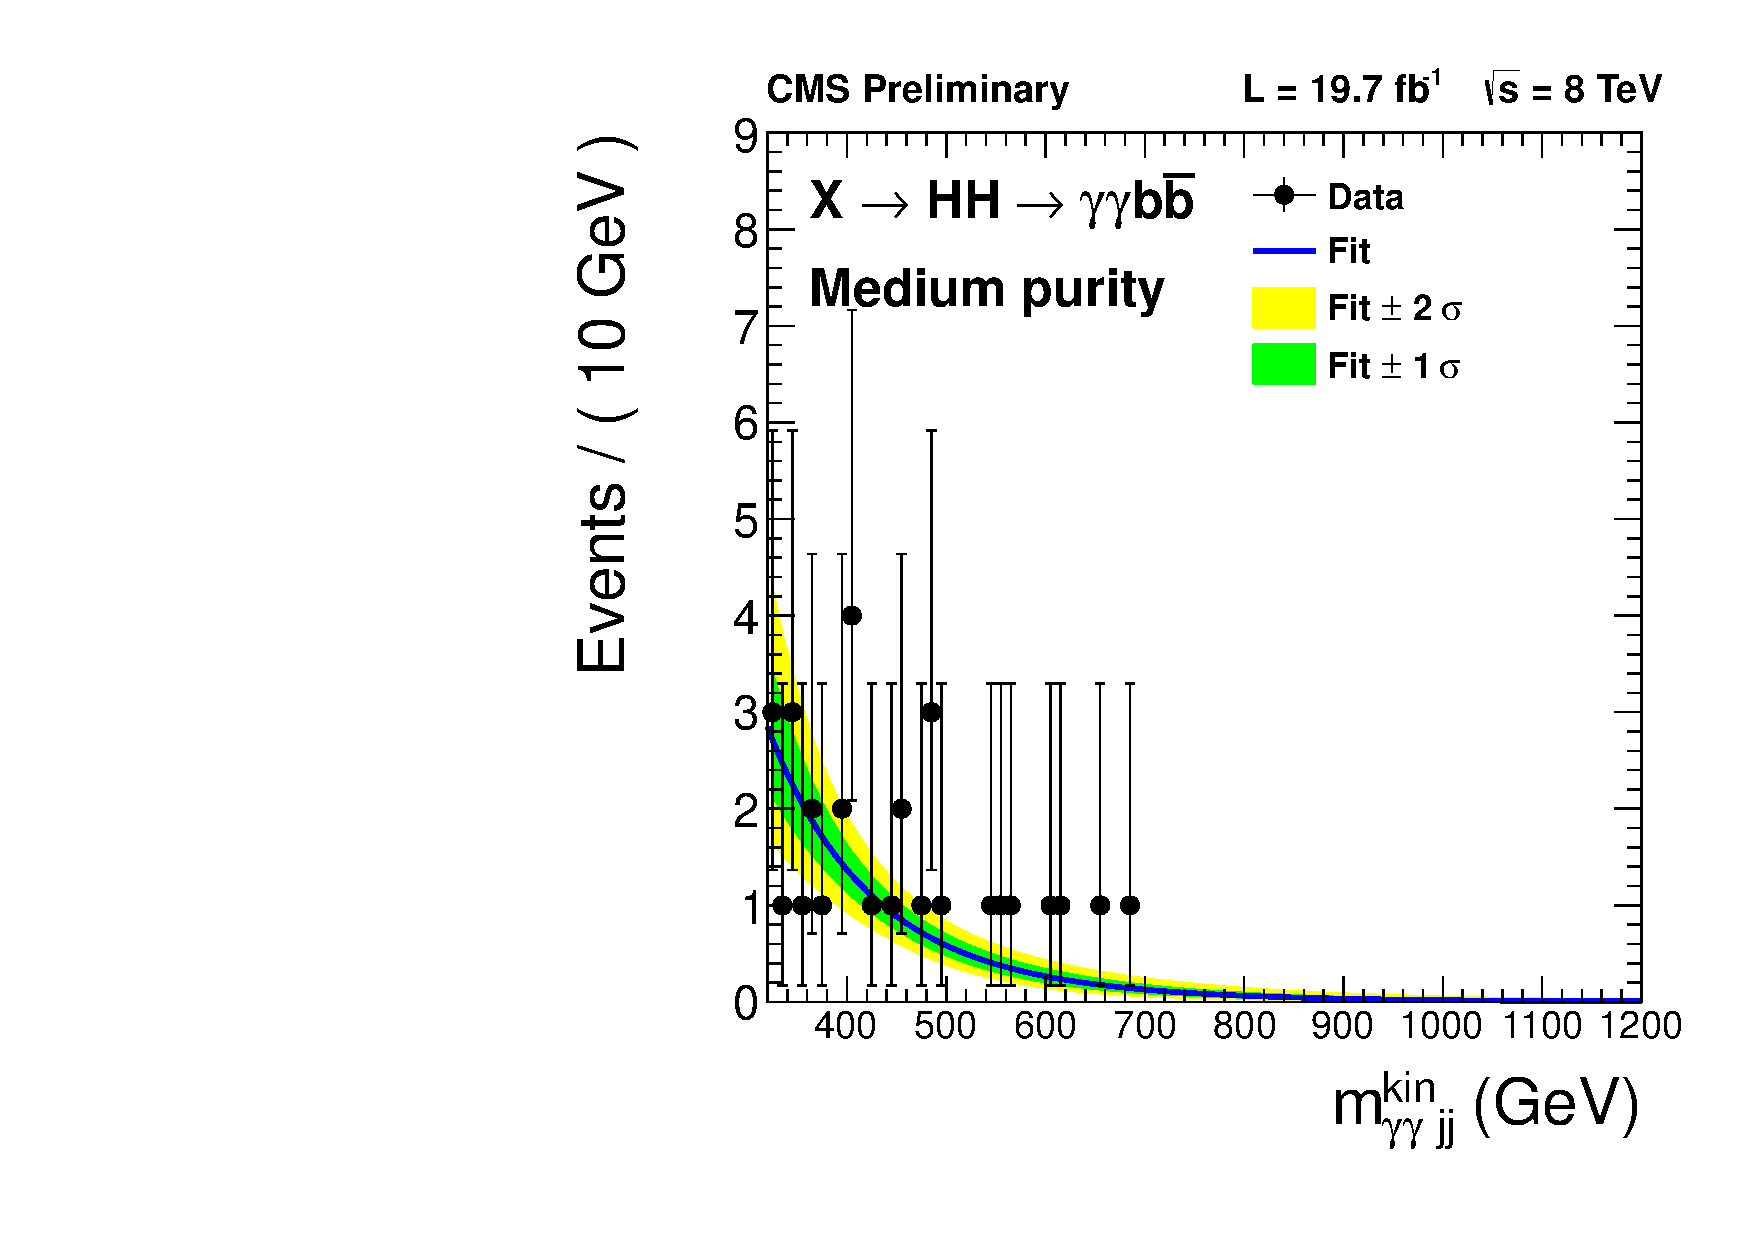
\includegraphics[width=0.70\textwidth]{figures/results/databkgoversig_cat1_4body.pdf}
 \end{center}
\caption{Events in the $\Mggjjk$ spectrum in the high-purity (top) and medium-purity (bottom)
categories. The background fit is shown in blue
with 1$\sigma$ and 2$\sigma$ bands on the background estimation.}
\label{fig:datafit_4body}
\end{figure}

There is no excess above the expection observed, so the analysis proceeds to calulating
upper limits on the signal cross section. The 95\% CL for expected and observed limits is
shown in Figure~\ref{fig:limits_allres}
for both categories and both mass regimes. The break at 400 GeV corresponds
to the border between both methods for signal extraction.
As in the low-mass regime, the theory expectations for the Radion assumes
$\text{BR}(R\rightarrow HH) =$~25\% for all Radion masses above 300 GeV. The result is again
spin-independent, allowing for both spin-0 and spin-2 theory expections to be overlaid together.

\begin{figure}[ht]
 \begin{center}
   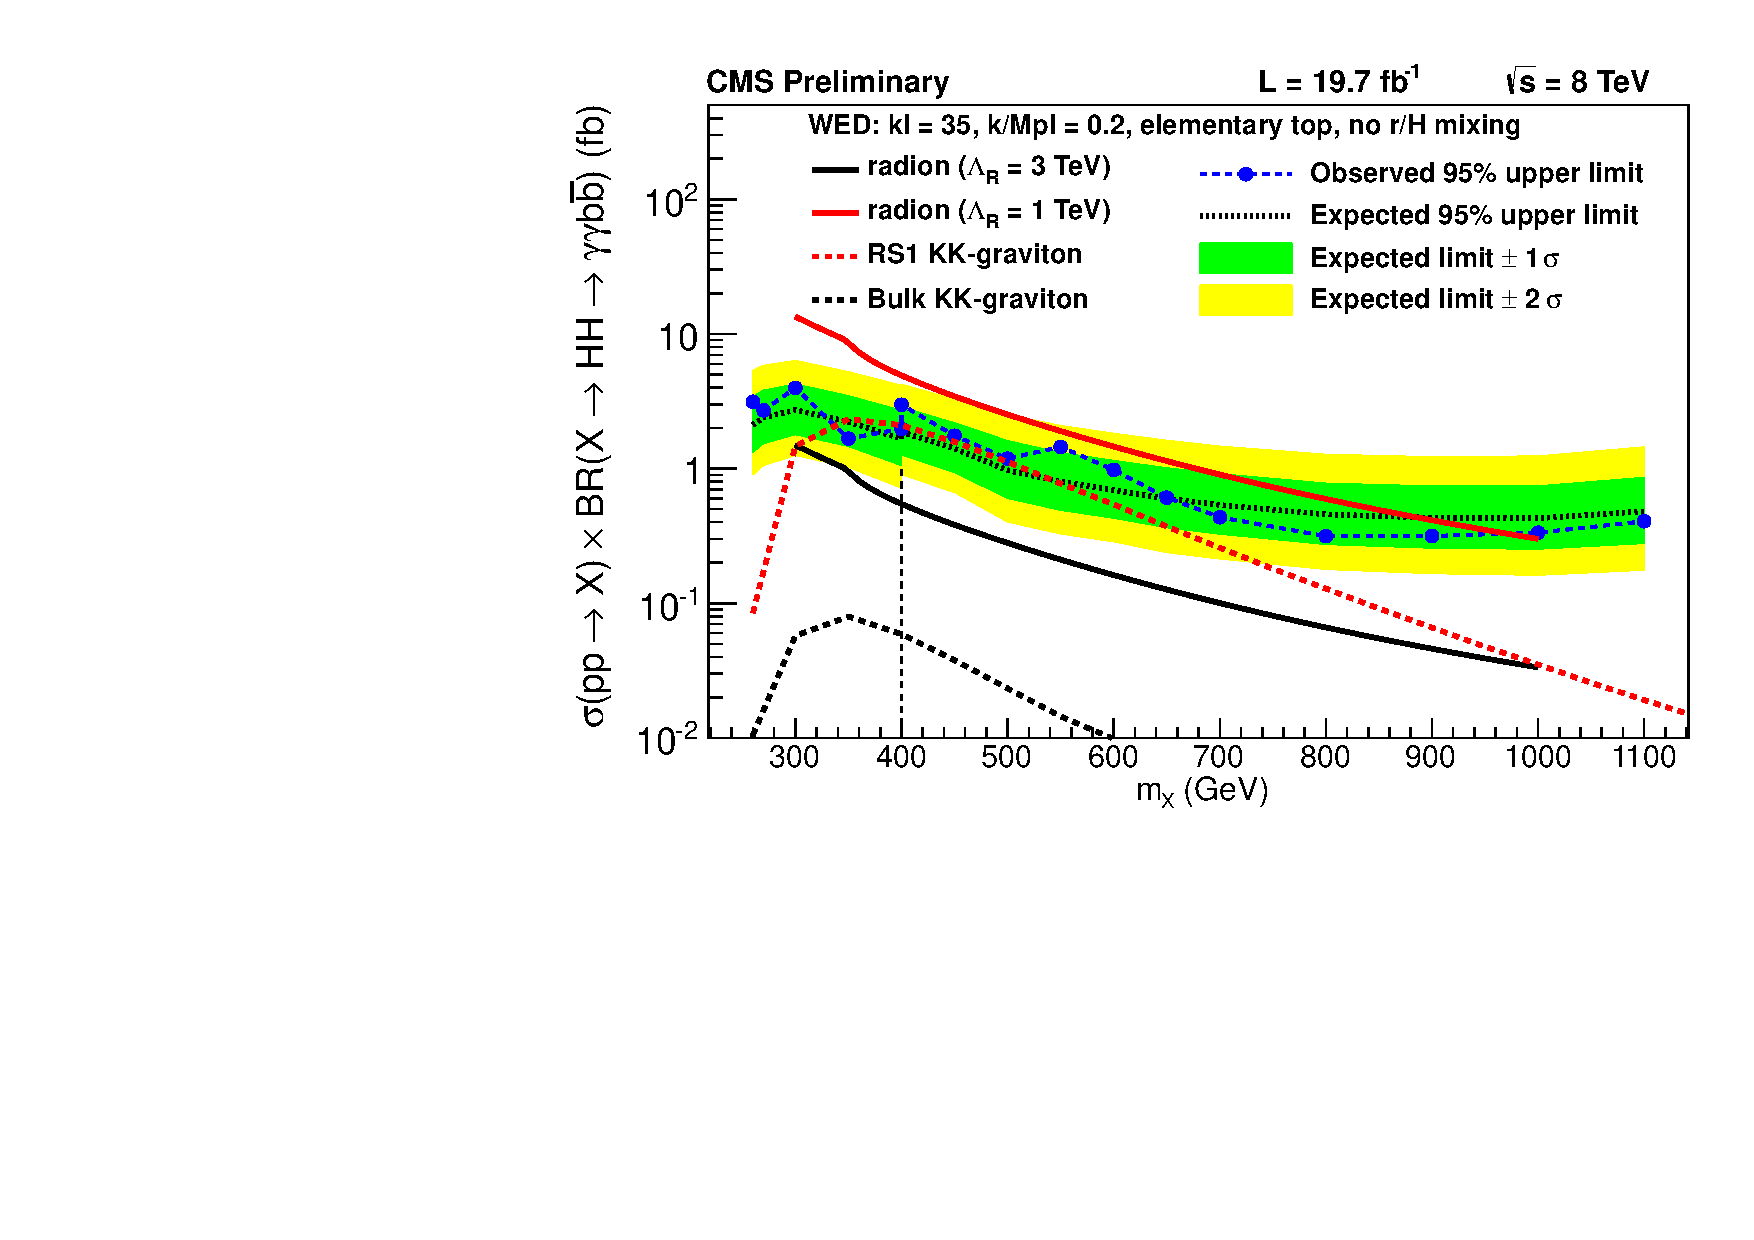
\includegraphics[width=0.7\textwidth]{figures/results/WP4_cutbased_all.pdf}
   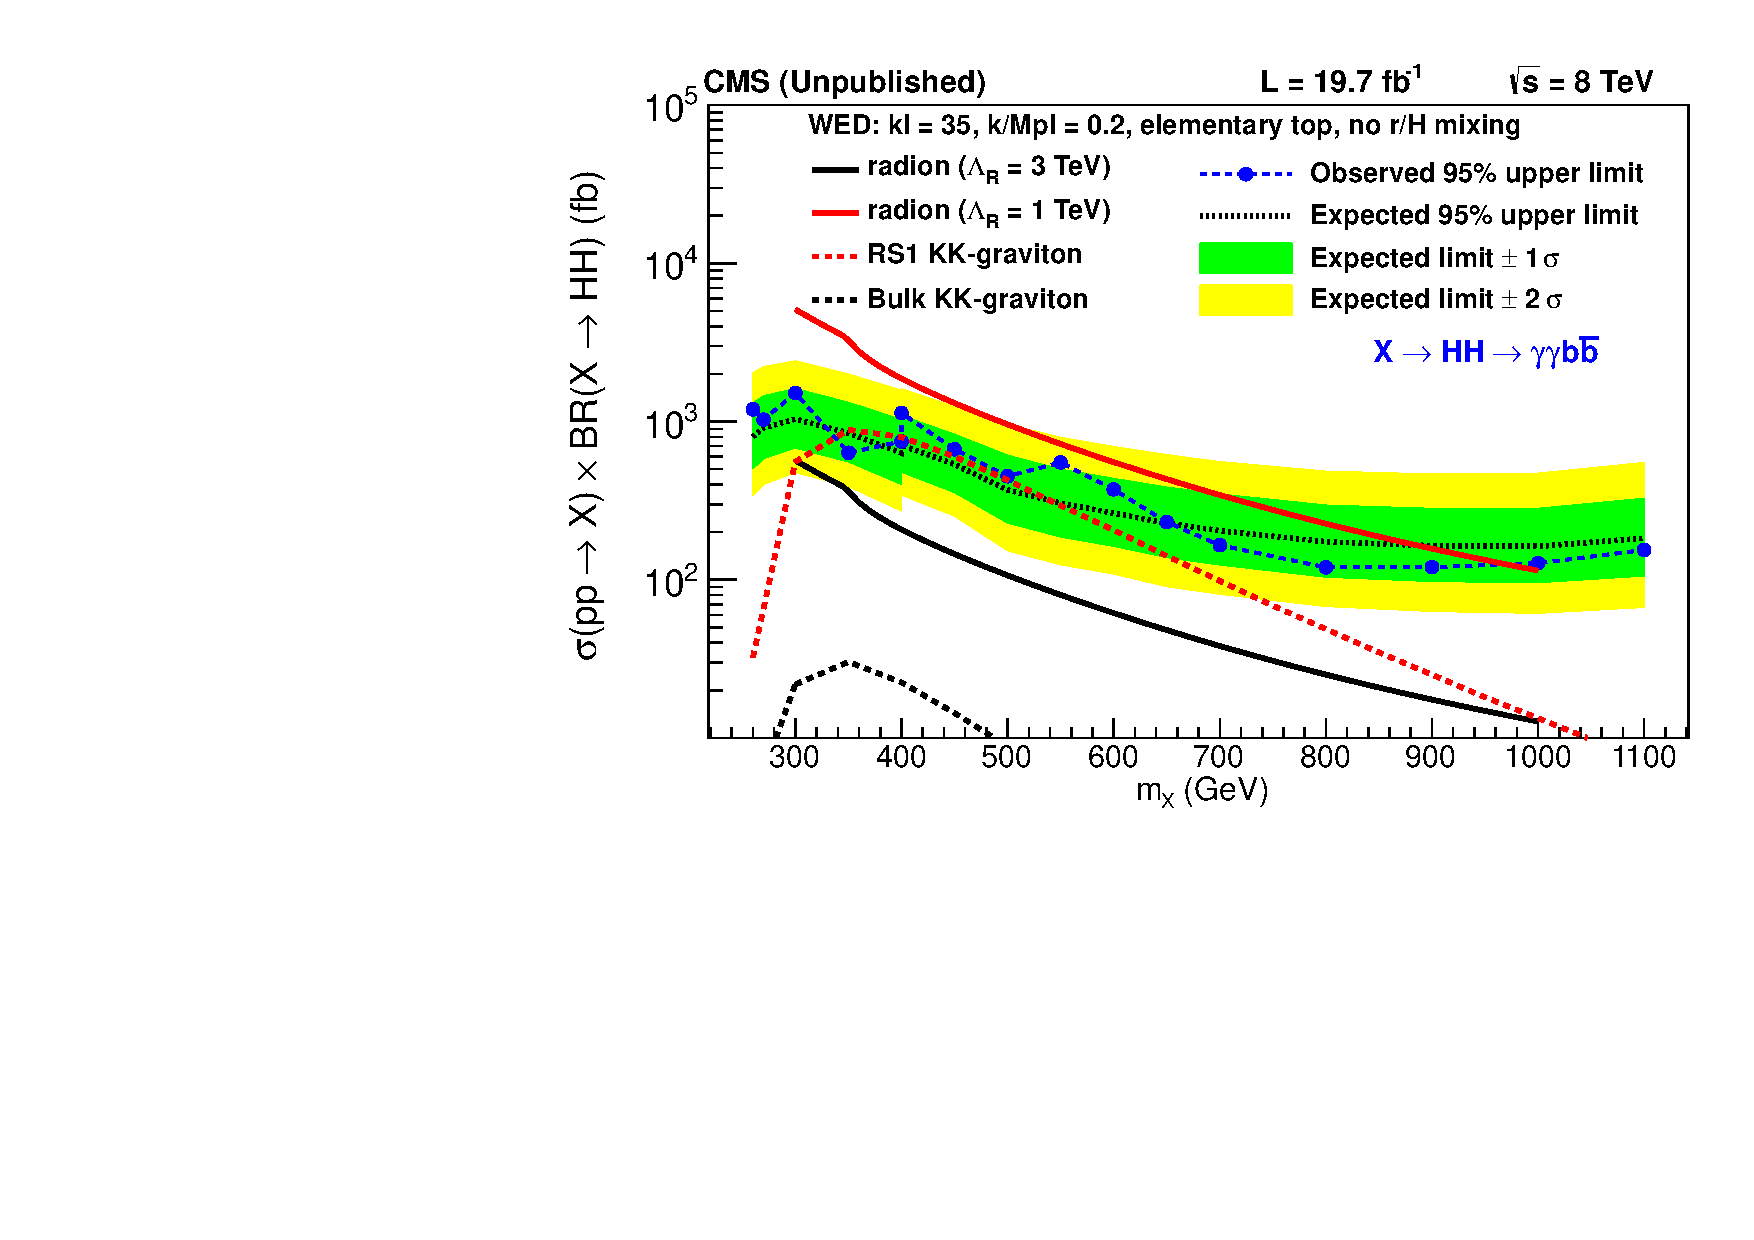
\includegraphics[width=0.7\textwidth]{figures/results/WP4_cutbased_HH.pdf}
 \end{center}
\caption{Expected 95\% CL upper limits on the cross section times branching ratios
$\sigma(pp\rightarrow X) \times \text{BR}( X \rightarrow HH \rightarrow \gamma\gamma b\bar{b})$ (top)
and $\sigma(pp\rightarrow X) \times \text{BR}( X \rightarrow HH )$ (bottom).
Theory lines corresponding to WED models with Radion, RS1 KK-graviton, and bulk KK-graviton are
overlaid. The results are obtained using the asymptotic $\text{CL}_s$ approach.}
\label{fig:limits_allres}
\end{figure}

Table~\ref{table:limits_highmass} and Figure~\ref{fig:limit_comp}
provide a comparison of the observed and expected limits obtained
among several final states in both the CMS and ATLAS Collaborations. The final states compared here
are $\gamma \gamma b\bar{b}$, $b\bar{b}b\bar{b}$, $\tau\tau b\bar{b}$, and multileptons and photons.
The comparison reveals that the $\gamma \gamma b\bar{b}$ is most sensitive to resonant double
Higgs production for $m_X < 400$~GeV, while the $b\bar{b}b\bar{b}$ final state is the most sensitive
for $m_X > 400$~GeV.

\begin{table}[ht]
  \centering
  \renewcommand{\arraystretch}{1.4}
  \caption{Observed and median expected 95\% CL upper limits for $m_X \ge 400$~GeV.}
  \begin{tabular}{ | c | c | c | }
\hline
$m_X$ (GeV) & Observed limit (fb) & Expected limit (fb) \\ \hline
400 & 2.98 & 1.87 \\
450 & 1.76 & 1.42 \\
500 & 1.19 & 0.97 \\
550 & 1.45 & 0.80 \\
600 & 0.98 & 0.69 \\
650 & 0.61 & 0.60 \\
700 & 0.44 & 0.54 \\
800 & 0.31 & 0.46 \\
900 & 0.32 & 0.43 \\
1000 & 0.33 & 0.43 \\
1100 & 0.41 & 0.48 \\ \hline
\end{tabular}

  \label{table:limits_highmass}
\end{table}

\begin{figure}[ht]
 \begin{center}
   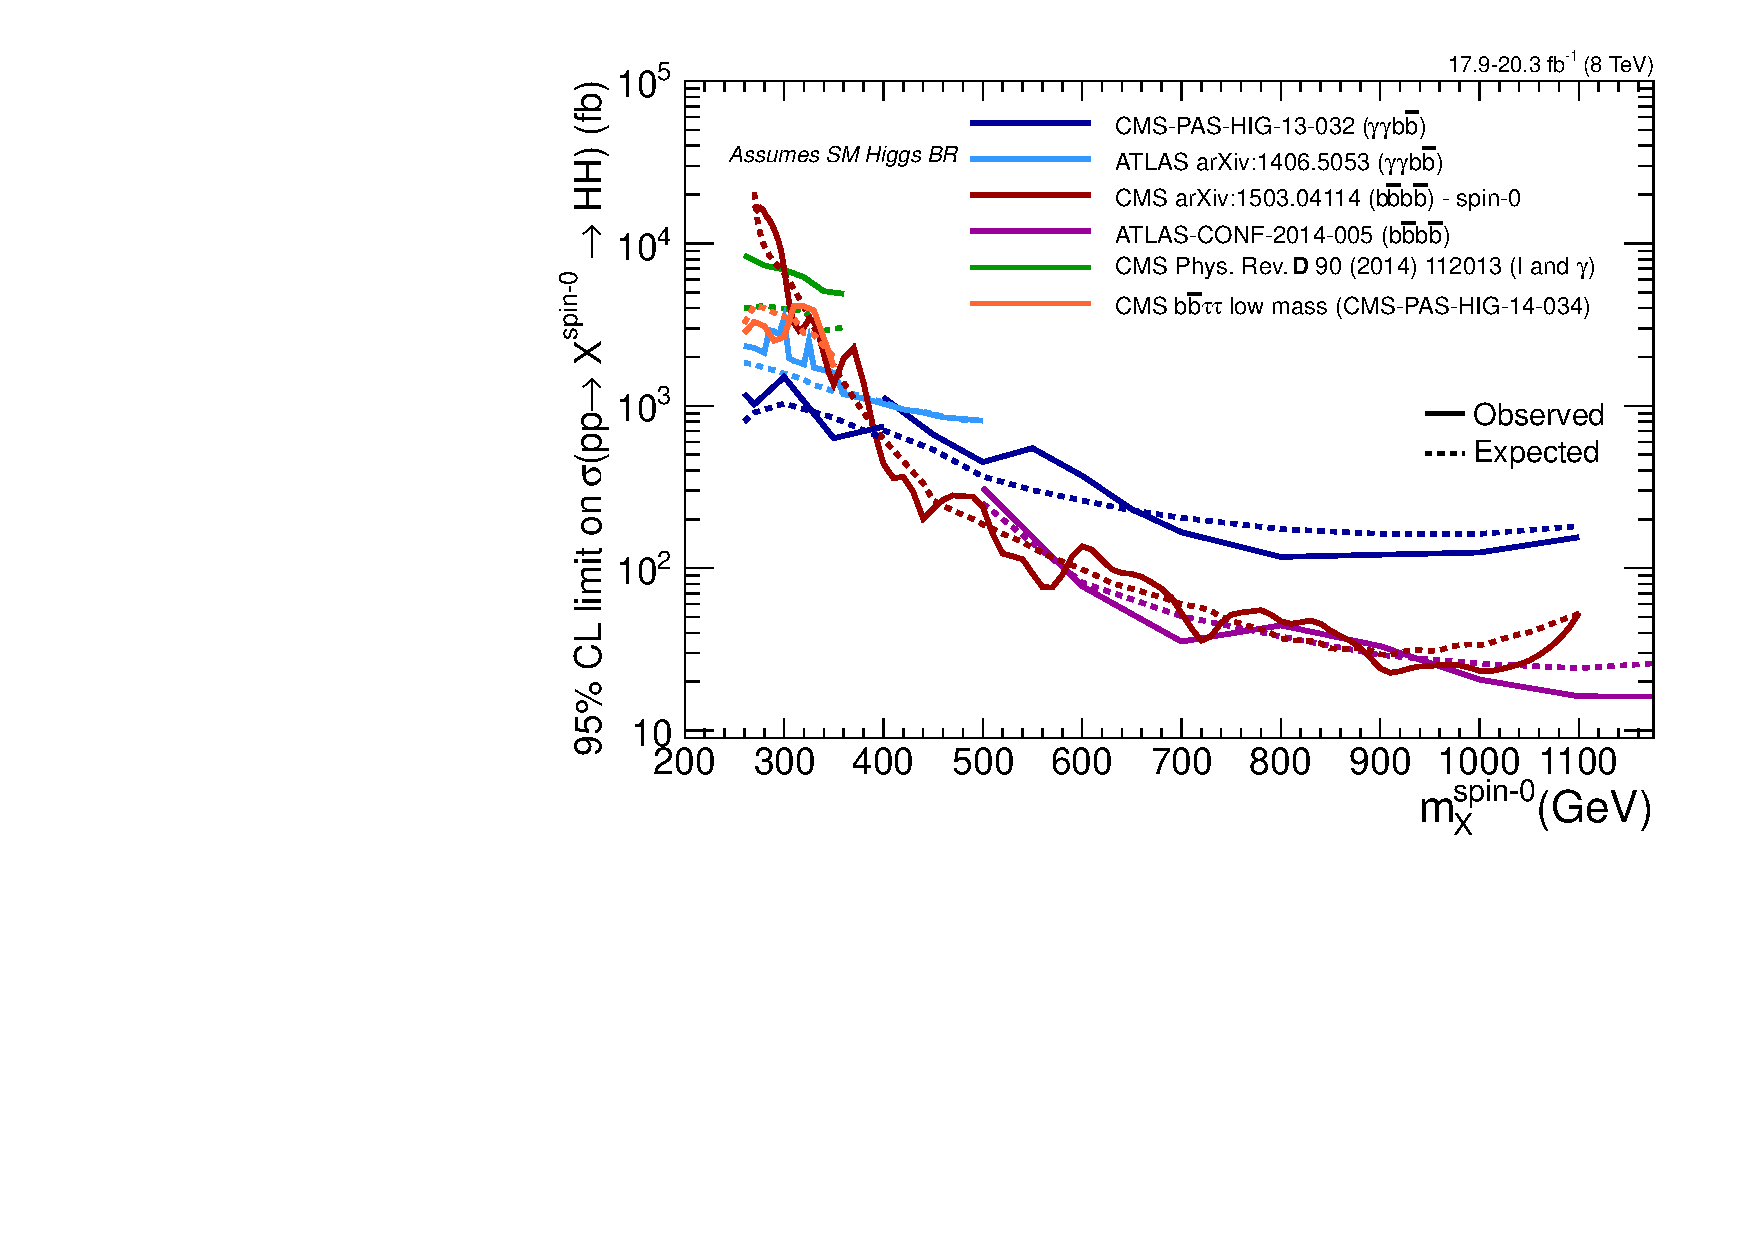
\includegraphics[width=0.8\textwidth]{figures/results/limit_comparison_all.pdf}
 \end{center}
\caption{The expected and observed upper limit of $X_\text{spin-0} \rightarrow HH$ production
at 95\% CL provided by combining the searches performed by the CMS and ATLAS experiments
looking at the $\gamma \gamma b\bar{b}$~\cite{CMS-PAS-HIG-13-032,Aad:2014yja},
$b\bar{b}b\bar{b}$~\cite{Khachatryan:2015yea,ATLAS-CONF-2014-005},
$\tau\tau b\bar{b}$~\cite{CMS-PAS-HIG-14-034}, and
multileptons and photons~\cite{PhysRevD.90.112013}
final states. As the CMS $b\bar{b}b\bar{b}$ result is dependent on the
resonance spin, the spin-0 result for that analysis is used.}
\label{fig:limit_comp}
\end{figure}


\section{Nonresonant Results\label{sec:nonresresults}}

For the SM nonresonant search, the signal yield is extracted by fitting the 2D plane
$\Mgg \times \Mjj$. The signal model is built by fitting simultaneous both dimensions separately
for the four categories. The functional form used in both dimensions is the sum of a Crystal Ball and
Gaussian with the means constrained to be the same. The background estimation is done by fitting
the same plane in each category on the interval $[100, 180]$~GeV for $\Mgg$ and $[60, 180]$~GeV
for $\Mjj$. The same bias estimation procedure
described for the low-mass resonant search is applied here. The chosen background function is a power
law for both dimensions in all four categories. The SM Higgs production is treated as a resonant
background, and its contribution on the final result is a few percent.

There is no excess above the expectation observed, so the analysis proceeds to calculating an
upper limit on the signal cross section. The 95\% CL is found using the same approach as both
regimes of the resonant search. The observed (expected) upper limit on SM
$pp \rightarrow HH \rightarrow \ggbb$ production cross section is 1.91 fb (1.59 fb).
Assuming SM Higgs branching ratios, the observed (expected) upper limit on SM $pp \rightarrow HH$
prodcution is 726 fb (604 fb). In terms of the SM signal strength modificator $\mu_{HH}$, defined as
\begin{equation}
\mu = \frac{\sigma}{\sigma_\text{SM}} \, ,
\end{equation}
the observed (expected) limit is 72.9 (60.7). These calculations accounted for the theoretical
uncertainty associated with the SM NNLO cross section.

%\section{The Future\label{sec:future}}

